\documentclass[conference]{IEEEtran}
\IEEEoverridecommandlockouts
% The preceding line is only needed to identify funding in the first footnote. If that is unneeded, please comment it out.
\usepackage{cite}
\usepackage{amsmath,amssymb,amsfonts,latexsym}
\usepackage{algorithmic}
\usepackage{graphicx}
\usepackage{subcaption}
\usepackage{textcomp}
\usepackage{xcolor}
\def\BibTeX{{\rm B\kern-.05em{\sc i\kern-.025em b}\kern-.08em
    T\kern-.1667em\lower.7ex\hbox{E}\kern-.125emX}}
% ---------------------

\usepackage{mathtools}
% \usepackage{amsthm, amssymb,latexsym}
% \usepackage{subfigure}
\usepackage{comment}
\usepackage{hyperref}
\usepackage{booktabs} % for professional tables
\usepackage{url}            % simple URL typesetting
\usepackage{multirow}

% *** GRAPHICS RELATED PACKAGES ***
%
\ifCLASSINFOpdf
  % \usepackage[pdftex]{graphicx}
  % declare the path(s) where your graphic files are
  % \graphicspath{{../pdf/}{../jpeg/}}
  % and their extensions so you won't have to specify these with
  % every instance of \includegraphics
  % \DeclareGraphicsExtensions{.pdf,.jpeg,.png}
\else
  % or other class option (dvipsone, dvipdf, if not using dvips). graphicx
  % will default to the driver specified in the system graphics.cfg if no
  % driver is specified.
  % \usepackage[dvips]{graphicx}
  % declare the path(s) where your graphic files are
  % \graphicspath{{../eps/}}
  % and their extensions so you won't have to specify these with
  % every instance of \includegraphics
  % \DeclareGraphicsExtensions{.eps}
\fi

% http://www.ctan.org/pkg/algorithmicx
\usepackage{titlesec}
\usepackage{makecell}
\usepackage{tikz}                                        
\usetikzlibrary{positioning, arrows.meta, fit, backgrounds, calc, shapes.geometric}


% correct bad hyphenation here
\hyphenation{op-tical net-works semi-conduc-tor}


\begin{document}
\title{Hail Quantum Hydra: Hybrid Quantum State Space Models for Long Sequence Learning \thanks{* These authors contributed equally.}}



% Concise form
\author{Junghoon Justin Park$^1$*, Yeonghyeon Park$^2$*, Jiook Cha$^{1,3,4}$\\
\small $^1$Interdisciplinary Program in Artificial Intelligence, Seoul National University \\ $^2$Department of Biosystems Engineering, Seoul National University \\ $^3$Department of Brain and Cognitive Sciences, Seoul National University $^4$Department of Psychology, Seoul National University \\
\small \texttt{utopie9090@snu.ac.kr, mandy1002@snu.ac.kr, connectome@snu.ac.kr}
}


% use for special paper notices
%\IEEEspecialpapernotice{(Invited Paper)}




% make the title area
\maketitle

\begin{abstract}

State Space Models such as Mamba and Hydra succeed by isolating sequence mixing as an explicit computational primitive. We ask whether this primitive can itself be enriched by operating in quantum Hilbert space.

Existing quantum sequence models do not localize mixing as a dedicated quantum primitive: in recurrent approaches (QRNN, QLSTM) it is buried inside state evolution, and in attention-based variants it is folded into the attention computation rather than separated as a localizable mixing step.

We propose Quantum Mamba and Quantum Hydra, hybrid models that apply quantum circuits at the SSM mixing step alone. Each chunk is evolved through three independent branches---forward, backward, and diagonal---whose states are coherently superposed at the amplitude level before measurement, generating interference cross-terms inaccessible to any classical mixture. The forward and backward branches let a learned scalar $\Delta$ modulate quantum rotation angles directly inside the circuit, bringing Mamba's input-dependent selectivity into the quantum domain; Quantum Hydra is the bidirectional extension with two such cores.

Across two EEG and two GLUE benchmarks, our models match or exceed classical Transformer, Mamba, and Hydra baselines: Quantum Hydra surpasses classical Hydra on PhysioNet by $0.082$ in test accuracy with $3.4\times$ fewer parameters and substantially tightens inter-seed variance on EEG, with gains largest in long-sequence and low-resource regimes.

\end{abstract}

% For peer review papers, you can put extra information on the cover

% page as needed:

% \ifCLASSOPTIONpeerreview

% \begin{center} \bfseries EDICS Category: 3-BBND \end{center}

% \fi

%

% For peerreview papers, this IEEEtran command inserts a page break and

% creates the second title. It will be ignored for other modes.

\IEEEpeerreviewmaketitle

\section{Introduction}

Sequence modeling has progressed rapidly with the advent of the Transformer architecture and its self-attention mechanism~\cite{Vaswani}. Despite their empirical success, Transformers suffer from quadratic computational and memory complexity in the sequence length, which limits their scalability to long-range dependencies in real-world data.

State Space Models (SSMs) such as Mamba~\cite{Gu2024} and Hydra~\cite{Hwang} address this limitation by reframing sequence modeling around \emph{mixing} as an explicit computational primitive: information propagation is selectively controlled by input-dependent dynamics~\cite{Gu2024} and, more generally, formalized as structured sequence mixers~\cite{Hwang}. This design achieves near-linear complexity while preserving fine-grained control over how and where information is aggregated.

In parallel, Quantum Machine Learning (QML) has been explored as a paradigm for leveraging the high-dimensional representational capacity of Hilbert spaces~\cite{Mishra2021QML, Tychola2023QMLoverview}. Embedding quantum computation into sequence modeling, however, remains challenging due to limited scalability, noise sensitivity, and trainability constraints on near-term devices~\cite{Lamichhane2025QML}.

Existing quantum sequence models do not localize mixing as an explicit primitive. Recurrent approaches such as QRNNs and QLSTMs encode temporal dependencies implicitly through quantum state evolution, so that mixing arises only as a byproduct of hidden-state propagation. More recent work, such as the Quantum Time-series Transformer~\cite{Park2025QTSTransformer}, places quantum computation inside the attention mechanism, delivering strong complexity reductions for the attention step itself but still embedding the mixing operation inside attention rather than isolating it as a dedicated, fixed-width primitive—the very design principle that has made modern classical SSMs successful.

The closest prior work is QMamba~\cite{Stenzel2025}, which translates Mamba's selective state space mechanism into a quantum setting by replacing its core operations with parameterized quantum circuits, preserving the A/B/C/$\Delta$ decomposition while enabling quantum-native state evolution. However, QMamba follows a single computational pathway in which the contributions of different transformation modes are entangled inside one unified circuit, leaving little room for explicitly composing distinct interaction patterns.

In contrast, we introduce a \emph{three-branch coherent superposition} mechanism in which each chunk representation is evolved through three independent quantum circuits—forward, backward, and diagonal—whose state vectors are combined at the amplitude level \emph{before} measurement. This structure directly mirrors the inductive biases of classical Hydra (selectivity and bidirectionality), while generating interference cross-terms of the form $\langle\psi_j|\hat{O}|\psi_k\rangle$ that are inaccessible to any classical convex combination of the individual branch measurements and absent in any single-branch quantum model.

To evaluate the effectiveness and generality of our approach, we conduct a systematic empirical study across multiple domains: physiological EEG (PhysioNet)~\cite{schalk2004bci2000,goldberger2000physiobank}, clinical EEG (ADFTD)~\cite{miltiadous2023dataset}, and natural language understanding (GLUE)~\cite{Wang2018GLUE}, with classical Transformer, Mamba, and Hydra baselines. Our results show that Quantum Mamba and Quantum Hydra achieve competitive performance while maintaining stable training dynamics under NISQ constraints, providing evidence that aligning state-space mixing with quantum interference is a productive direction for scalable quantum sequence learning, and more broadly that isolating the right computational primitive is a practical route to quantum-enhanced learning.

\section{Background}

\subsection{State Space Models for Sequence Modeling}

Early sequence models based on recurrent neural networks struggled to capture long-range dependencies due to vanishing gradients and sequential computation bottlenecks~\cite{Hochreiter1997}. The Transformer architecture addressed this through global self-attention, but at the cost of quadratic complexity with respect to sequence length~\cite{Vaswani}. State Space Models (SSMs) emerged as a principled alternative, reformulating sequence dynamics as continuous-time latent state transitions that can be discretized and computed as linear convolutions, achieving near-linear complexity~\cite{Gu2021S4, Somvanshi2025SSMSurvey}.

Early SSMs such as S4~\cite{Gu2021S4} demonstrated that structured parameterizations of state matrices enable efficient long-range modeling via convolutional computation. Subsequent models including H3~\cite{Fu2022H4} and Hyena~\cite{Poli2023Hyena} extended this framework with multiplicative interactions and implicit long convolutions, progressively closing the performance gap with attention-based models. However, these models share a common limitation: their state-space parameters are fixed across inputs, making them linear time-invariant systems that cannot adapt their information aggregation to the content of the sequence.

\subsubsection{Mamba: Selective State Space Models}

Mamba addresses this limitation by introducing input-dependent state-space parameters $(\Delta, B, C)$ that vary with each token~\cite{Gu2023Mamba}. Concretely, the discretization factor $\Delta$ controls how much of the current input is absorbed into the hidden state at each step, acting as a learned, content-aware gate over temporal information. When $\Delta \to 0$, the model effectively ignores the current token; when $\Delta \to 1$, the full input is integrated into the state. This selectivity allows Mamba to focus on task-relevant tokens while suppressing noise—a capability fundamentally absent in earlier linear time-invariant SSMs. Combined with a hardware-aware parallel scan algorithm, Mamba achieves $\mathcal{O}(N)$ complexity while matching or exceeding Transformer performance across multiple modalities~\cite{Gu2023Mamba}.

\subsubsection{Hydra: Bidirectional Selective Mixing}

While Mamba's selectivity enables powerful causal sequence modeling, its unidirectional structure limits its applicability to tasks requiring full-context understanding. Hydra addresses this by extending selective SSMs to both temporal directions~\cite{Hwang2024Hydra}. Specifically, Hydra maintains two parallel selective SSM streams—one processing the sequence causally (left to right) and one anti-causally (right to left)—whose outputs are fused via a generalized matrix mixer. This bidirectional structure enables simultaneous access to past and future context, which is critical for classification and semantic understanding tasks where labels depend on the full sequence rather than its causal prefix. Crucially, Hydra demonstrates that SSM-based linear mixers, when equipped with both selectivity and bidirectionality, can match the representational capacity of attention-based encoders such as BERT~\cite{devlin2019bert}, while maintaining sub-quadratic complexity~\cite{Hwang2024Hydra}.

Taken together, the trajectory from S4 to Mamba and Hydra reflects a clear architectural trend: progressively enriching the \textit{mixing primitive}—the core operation responsible for aggregating information across the sequence—with selectivity and bidirectionality, while preserving linear scalability.

\subsubsection{Toward Quantum-Enhanced Mixing}

Despite their efficiency, classical SSM mixers operate within a fixed Euclidean feature space, aggregating sequence information through structured linear transformations. This raises a natural question: can the mixing primitive be further enriched by operating in a fundamentally different computational space?

Motivated by this, we explore \textit{quantum-coherent mixing} as a complementary paradigm. Variational quantum circuits (VQCs) embed classical data into an exponentially large Hilbert space~\cite{Schuld2022}, where interactions are governed by phase-sensitive interference rather than explicit linear combinations. This offers a qualitatively different mechanism for encoding dependencies: rather than computing weighted sums of feature vectors, quantum mixing operates over superposed amplitude distributions, generating cross-terms that have no direct classical analogue~\cite{havlicek2019supervised, Schuld2022}.

Our hybrid architectures—Quantum Mamba and Quantum Hydra—retain the linear scalability and inductive biases of their classical counterparts, while replacing the classical mixing primitive with a quantum-coherent counterpart. The three-branch coherent superposition structure directly inherits the forward, backward, and diagonal components of classical Hydra, reexpressing their inductive biases through quantum interference rather than structured linear algebra. 

% \subsection{Variational Quantum Circuits for Machine Learning}

% With the advent of the Noisy Intermediate-Scale Quantum (NISQ) era, Variational Quantum Circuits (VQCs), which combine classical optimization loops with parameterized quantum circuits, have become a central tool in quantum machine learning. VQCs map features into high-dimensional Hilbert spaces by leveraging quantum principles such as superposition and entanglement. Recent theoretical and empirical studies have hypothesized that such VQC architectures may offer richer representations and enhanced generalization performance for certain structured data compared to classical neural networks.

\subsection{Variational quantum circuits}
Variational quantum circuits (VQCs) are a foundational paradigm of quantum machine learning (QML) that bridges classical computational tasks and quantum computation. A VQC typically consists of three components: an encoding circuit, a parameterized ansatz circuit, and a measurement stage.

The encoding circuit $U(\overrightarrow{x})$ maps a classical input vector $\overrightarrow{x}$ into a quantum state $U(\overrightarrow{x})|0\rangle^{\otimes n}$, where $|0\rangle^{\otimes n}$ is the initial ground state of an $n$-qubit system. This embedding lifts classical data into the exponentially large Hilbert space $\mathbb{C}^{2^n}$, which is the key resource for potential quantum advantage.

The encoded state is then transformed by a parameterized ansatz circuit $W(\Theta)$ composed of $M$ trainable layers, producing the state
\begin{align}
    |\psi(\overrightarrow{x}, \Theta)\rangle = W(\Theta)U(\overrightarrow{x})|0\rangle^{\otimes n} \nonumber \\ = \left(\prod_{j=M}^{1} V_j(\overrightarrow{\theta_j})\right)U(\overrightarrow{x})|0\rangle^{\otimes n},
\label{QuantumState}
\end{align}
where each layer $V_j(\overrightarrow{\theta_j})$ is parameterized by $\overrightarrow{\theta_j}$, and $\Theta=\{\overrightarrow{\theta_1}, \ldots, \overrightarrow{\theta_M}\}$ collects all trainable parameters. A layer typically consists of single-qubit rotation gates followed by two-qubit entangling gates, enabling the circuit to represent a rich class of quantum states.

Information is extracted from the resulting state through quantum measurements of chosen observables $\hat{H}_k$. These observables are Hermitian operators ($\hat{H}_k=\hat{H}_k^\dagger$), which guarantees real-valued expectation values and is essential for interfacing with classical loss functions. The VQC thus implements a quantum parametric function
\begin{equation}
\overrightarrow{f}(\overrightarrow{x}; \Theta) = \left(\langle \hat{H}_1 \rangle, \ldots, \langle \hat{H}_n \rangle\right),
\end{equation}
whose components are given by
\begin{equation}
\langle \hat{H}_k \rangle = \langle 0|U^{\dagger}(\overrightarrow{x})W^{\dagger}(\Theta)\hat{H}_k W(\Theta)U(\overrightarrow{x})|0\rangle.
\end{equation}
In practice, these expectation values are estimated from repeated measurements (shots) on quantum hardware, or computed exactly on classical simulators.

During training, the parameters $\Theta$ are iteratively updated to minimize a task-specific loss function $\mathcal{L}(\overrightarrow{x}, y; \Theta)$ over a training set $D=\{(\overrightarrow{x}_i, y_i)\}_i$. For regression, a typical choice is
\begin{equation}
\mathcal{L}(\overrightarrow{x}, y; \Theta) = \sum_i \| f_{\Theta}(\overrightarrow{x}_i) - y_i \|^2.
\end{equation}
The loss (or its gradient) is estimated from the circuit outputs and passed to a classical optimizer that solves
\begin{equation}
\arg\min_{\Theta}\mathcal{L}(\overrightarrow{x},y; \Theta).
\end{equation}

In many applications, it is also useful to treat the measurement observable itself as learnable. Any Hermitian operator $H$ on an $n$-qubit system can be written in the elementary-matrix basis as
\begin{equation}
    H = \sum_{i,j=1}^{N} h_{ij}E_{ij}, \quad h_{ij}=\overline{h_{ji}}, \quad N=2^n,
\end{equation}
where $E_{ij}$ has a single nonzero entry at position $(i,j)$, i.e., $(E_{ij})_{kl}=\delta_{ik}\delta_{jl}$. Parameterizing $H$ by the coefficients $\overrightarrow{h}$, the expectation value with respect to the state in Eq.~\eqref{QuantumState} becomes linear in $\overrightarrow{h}$:
\begin{equation}
    \langle\psi|H(\overrightarrow{h})|\psi\rangle = \sum_{i,j=1}^{N}h_{ij}\langle\psi|E_{ij}|\psi\rangle.
\end{equation}
Its gradient with respect to each coefficient takes the particularly clean form
\begin{align}
    \frac{\partial \langle\psi|H(\overrightarrow{h})|\psi\rangle}{\partial h_{kl}} &= \langle\psi|E_{kl}|\psi\rangle \nonumber \\
    &= \left(\overline{W(\Theta)U(\overrightarrow{x})}\right)_{k1}\left(W(\Theta)U(\overrightarrow{x})\right)_{l1},
\end{align}
which makes the joint dependence on the parameterized circuit $W(\Theta)$ and the encoded data $U(\overrightarrow{x})$ explicit.

In summary, VQCs provide a flexible, end-to-end differentiable framework that leverages quantum phenomena such as superposition and entanglement, and can be seamlessly embedded as differentiable modules within larger classical deep learning pipelines.


\subsection{Quantum Sequence Models}

Prior work on quantum sequence modeling can be broadly categorized into two paradigms, depending on how temporal dependencies and mixing are formulated.

One line of work builds on recurrent architectures. Quantum RNNs~\cite{Bausch2020QRNN, Li2023QRNN} maintain a quantum state that is unitarily evolved across timesteps, while Quantum LSTMs~\cite{Chen2022QLSTM} replace classical gating mechanisms with variational quantum circuits within a recurrent backbone. In these approaches, temporal dependencies are encoded implicitly through state evolution, and mixing arises as a byproduct of hidden-state propagation rather than as an explicit operation. As a result, these models inherit well-known limitations of classical recurrent architectures, including difficulty in capturing long-range dependencies~\cite{Hochreiter1997RNN}, and do not provide mechanisms for selective or bidirectional information aggregation.

A second line of work attempts to model mixing explicitly via global quantum operations within an attention backbone. The recently proposed Quantum Time-series Transformer (QTSTransformer)~\cite{Park2025QTSTransformer} replaces the classical Q/K/V attention computation with a quantum module combining Linear Combination of Unitaries (LCU) and Quantum Singular Value Transformation (QSVT)~\cite{Childs2017lineareq, Gilyen2019QSTT}, achieving polylogarithmic complexity in the attention step while preserving the transformer's scalability principles. To remain compatible with near-term hardware, QTSTransformer chunks the input sequence into temporal windows and applies the LCU+QSVT module within each window, with Pauli expectation values forming the resulting attention features; this design has been validated on resting-state fMRI biomarker discovery. Despite these advances, the LCU+QSVT formulation still requires block-encodings of the input and polynomial approximations of nonlinear transformations, so that circuit depth grows with both window length and approximation degree~\cite{Tomal2025QAttentionNLP, Kuznetsov2026QAttentionLLM}. As the authors of QTSTransformer themselves acknowledge, this scaling exposes the model to NISQ-era depth limits and to optimization pathologies such as barren plateaus, where gradients vanish exponentially with circuit depth~\cite{McClean2018, Larocca2025, Cerezo2021}.

These observations motivate our approach: rather than applying quantum computation globally or implicitly, we introduce quantum-coherent mixing as a localized module aligned with the SSM mixing primitive.

\section{Methods}
\label{sec:methods}

We propose two hybrid quantum-classical architectures for sequence classification: \textbf{Quantum Mamba}, a unidirectional model, and \textbf{Quantum Hydra}, its bidirectional extension.
Both models share the same core design: a classical encoder projects temporal inputs into a latent space and partitions them into chunks, and a parameterized quantum circuit then mixes each chunk by \emph{coherently superposing} three independently evolved branch states at the amplitude level, exploiting interference effects that cannot be reproduced by classical mixtures of measurement outcomes.
Throughout, we denote the number of qubits by $n$, the number of variational layers by $L$, the model hidden dimension by $d$, and the chunk size by $C$.

% ============================================================
\subsection{Quantum Mamba}
\label{sec:quantum_mamba}

Quantum Mamba processes a sequence $\mathbf{X} \in \mathbb{R}^{B \times T \times F}$ (batch $B$, $T$ timesteps, $F$ channels) in three stages: (i)~a classical encoder that produces chunk-level summaries, (ii)~a three-branch coherent quantum core that mixes each chunk, and (iii)~a classical aggregator and classifier.
Fig.~\ref{fig:qmamba_architecture} shows the overall architecture.

% ============================================================
% Quantum Mamba architecture diagram (TikZ)
% Include in main document with:
%   \usepackage{tikz}
%   \usetikzlibrary{positioning, arrows.meta, fit, backgrounds, calc, shapes.geometric}
%   % ============================================================
% Quantum Mamba architecture diagram (TikZ)
% Include in main document with:
%   \usepackage{tikz}
%   \usetikzlibrary{positioning, arrows.meta, fit, backgrounds, calc, shapes.geometric}
%   % ============================================================
% Quantum Mamba architecture diagram (TikZ)
% Include in main document with:
%   \usepackage{tikz}
%   \usetikzlibrary{positioning, arrows.meta, fit, backgrounds, calc, shapes.geometric}
%   \input{fig_quantum_mamba.tex}
% ============================================================

\begin{figure*}[t]
\centering
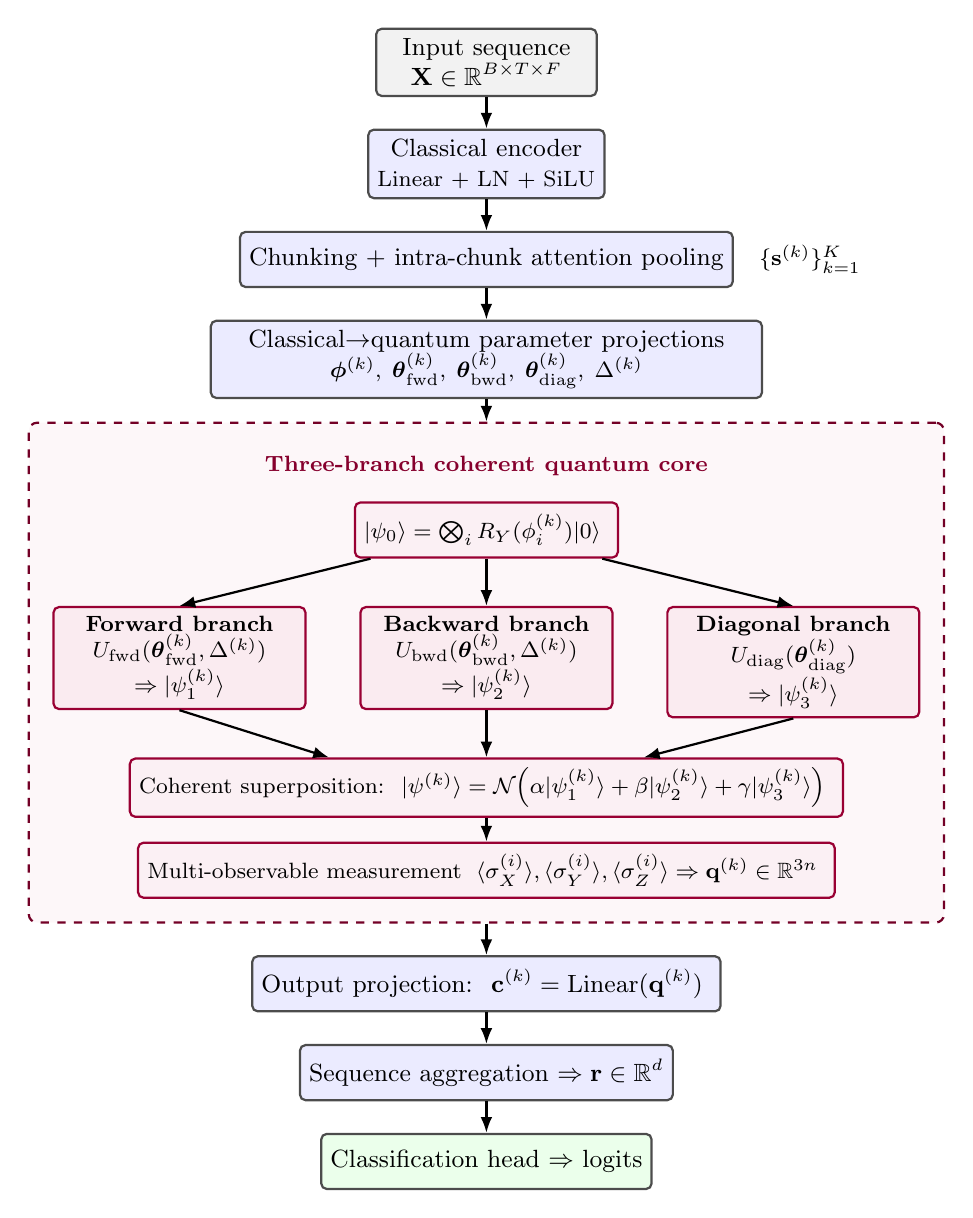
\begin{tikzpicture}[
    font=\small,
    node distance=4mm and 6mm,
    >=Latex,
    classical/.style={
        rectangle, rounded corners=2pt,
        draw=black!70, thick,
        fill=blue!8,
        minimum width=28mm, minimum height=7mm,
        align=center
    },
    cbranch/.style={
        rectangle, rounded corners=2pt,
        draw=black!70, thick,
        fill=blue!8,
        minimum width=22mm, minimum height=6mm,
        align=center, font=\footnotesize
    },
    qbranch/.style={
        rectangle, rounded corners=2pt,
        draw=purple!80!black, thick,
        fill=purple!8,
        minimum width=32mm, minimum height=9mm,
        align=center, font=\footnotesize
    },
    qcore/.style={
        rectangle, rounded corners=2pt,
        draw=purple!80!black, thick,
        fill=purple!6,
        minimum width=28mm, minimum height=7mm,
        align=center, font=\footnotesize
    },
    tensor/.style={font=\footnotesize\itshape},
    arrow/.style={-{Latex[length=2mm]}, thick},
]

% ---------- Input ----------
\node[classical, fill=gray!10] (input) {Input sequence\\$\mathbf{X} \in \mathbb{R}^{B \times T \times F}$};

% ---------- Classical encoder ----------
\node[classical, below=of input] (encoder) {Classical encoder\\\footnotesize Linear $+$ LN $+$ SiLU};

% ---------- Chunking ----------
\node[classical, below=of encoder] (chunk) {Chunking $+$ intra-chunk attention pooling};
\node[tensor, right=2mm of chunk] {$\{\mathbf{s}^{(k)}\}_{k=1}^{K}$};

% ---------- C→Q projections ----------
\node[classical, below=of chunk, minimum width=70mm] (proj) {%
    Classical$\to$quantum parameter projections\\%
    \footnotesize $\boldsymbol{\phi}^{(k)},\;\boldsymbol{\theta}_{\text{fwd}}^{(k)},\;\boldsymbol{\theta}_{\text{bwd}}^{(k)},\;\boldsymbol{\theta}_{\text{diag}}^{(k)},\;\Delta^{(k)}$
};

% ---------- Quantum core (big box) ----------
% Title above the branches
\node[below=6mm of proj, font=\footnotesize\bfseries, text=purple!70!black] (coretitle)
    {Three-branch coherent quantum core};

% Input encoding
\node[qcore, below=2mm of coretitle] (enc) {%
    $|\psi_0\rangle = \bigotimes_i R_Y(\phi_i^{(k)})|0\rangle$
};

% Three branches side by side
\node[qbranch, below left=6mm and 6mm of enc] (fwd) {%
    \textbf{Forward branch}\\%
    $U_{\text{fwd}}(\boldsymbol{\theta}_{\text{fwd}}^{(k)},\Delta^{(k)})$\\%
    $\Rightarrow |\psi_1^{(k)}\rangle$
};
\node[qbranch, below=6mm of enc] (bwd) {%
    \textbf{Backward branch}\\%
    $U_{\text{bwd}}(\boldsymbol{\theta}_{\text{bwd}}^{(k)},\Delta^{(k)})$\\%
    $\Rightarrow |\psi_2^{(k)}\rangle$
};
\node[qbranch, below right=6mm and 6mm of enc] (diag) {%
    \textbf{Diagonal branch}\\%
    $U_{\text{diag}}(\boldsymbol{\theta}_{\text{diag}}^{(k)})$\\%
    $\Rightarrow |\psi_3^{(k)}\rangle$
};

% Coherent superposition
\node[qcore, below=6mm of bwd, minimum width=75mm] (super) {%
    Coherent superposition:\; $|\psi^{(k)}\rangle = \mathcal{N}\!\left(\alpha|\psi_1^{(k)}\rangle + \beta|\psi_2^{(k)}\rangle + \gamma|\psi_3^{(k)}\rangle\right)$
};

% Measurement
\node[qcore, below=3mm of super, minimum width=75mm] (meas) {%
    Multi-observable measurement\; $\langle\sigma_X^{(i)}\rangle,\langle\sigma_Y^{(i)}\rangle,\langle\sigma_Z^{(i)}\rangle \Rightarrow \mathbf{q}^{(k)} \in \mathbb{R}^{3n}$
};

% Bounding box for the core
\begin{pgfonlayer}{background}
\node[
    draw=purple!60!black, thick, dashed, rounded corners=3pt,
    fill=purple!3,
    fit=(coretitle)(enc)(fwd)(diag)(super)(meas),
    inner sep=3mm
] (qcoreBox) {};
\end{pgfonlayer}

% ---------- Output projection ----------
\node[classical, below=4mm of qcoreBox] (outproj) {%
    Output projection:\; $\mathbf{c}^{(k)} = \mathrm{Linear}(\mathbf{q}^{(k)})$
};

% ---------- Sequence aggregation ----------
\node[classical, below=of outproj] (seqagg) {Sequence aggregation $\Rightarrow \mathbf{r} \in \mathbb{R}^{d}$};

% ---------- Classifier ----------
\node[classical, below=of seqagg, fill=green!8] (cls) {Classification head $\Rightarrow$ logits};

% ---------- Arrows ----------
\draw[arrow] (input) -- (encoder);
\draw[arrow] (encoder) -- (chunk);
\draw[arrow] (chunk) -- (proj);
\draw[arrow] (proj) -- (qcoreBox.north);

\draw[arrow] (enc) -- (fwd.north);
\draw[arrow] (enc) -- (bwd);
\draw[arrow] (enc) -- (diag.north);

\draw[arrow] (fwd.south) -- ([xshift=-20mm]super.north);
\draw[arrow] (bwd.south) -- (super.north);
\draw[arrow] (diag.south) -- ([xshift=20mm]super.north);

\draw[arrow] (super) -- (meas);
\draw[arrow] (qcoreBox.south) -- (outproj);
\draw[arrow] (outproj) -- (seqagg);
\draw[arrow] (seqagg) -- (cls);

\end{tikzpicture}
\caption{%
\textbf{Quantum Mamba architecture.}
A classical encoder projects the input sequence $\mathbf{X}$ and partitions it into chunks, each summarized by intra-chunk attention pooling.
For each chunk, the summary $\mathbf{s}^{(k)}$ is mapped through separate linear projections to the quantum input angles $\boldsymbol{\phi}^{(k)}$, three sets of variational parameters $\{\boldsymbol{\theta}_{\text{fwd}}^{(k)}, \boldsymbol{\theta}_{\text{bwd}}^{(k)}, \boldsymbol{\theta}_{\text{diag}}^{(k)}\}$, and a scalar selective-gating factor $\Delta^{(k)}$.
Three independent quantum branches (forward and backward Delta-modulated, diagonal unmodulated) are evolved from the same input state $|\psi_0\rangle$ and coherently combined at the amplitude level through learnable complex coefficients $\alpha, \beta, \gamma$ before multi-observable measurement.
The resulting chunk-level quantum feature vectors $\mathbf{q}^{(k)}$ are then projected back to the model hidden space, aggregated across chunks, and passed through a classification head.%
}
\label{fig:qmamba_architecture}
\end{figure*}

% ============================================================

\begin{figure*}[t]
\centering
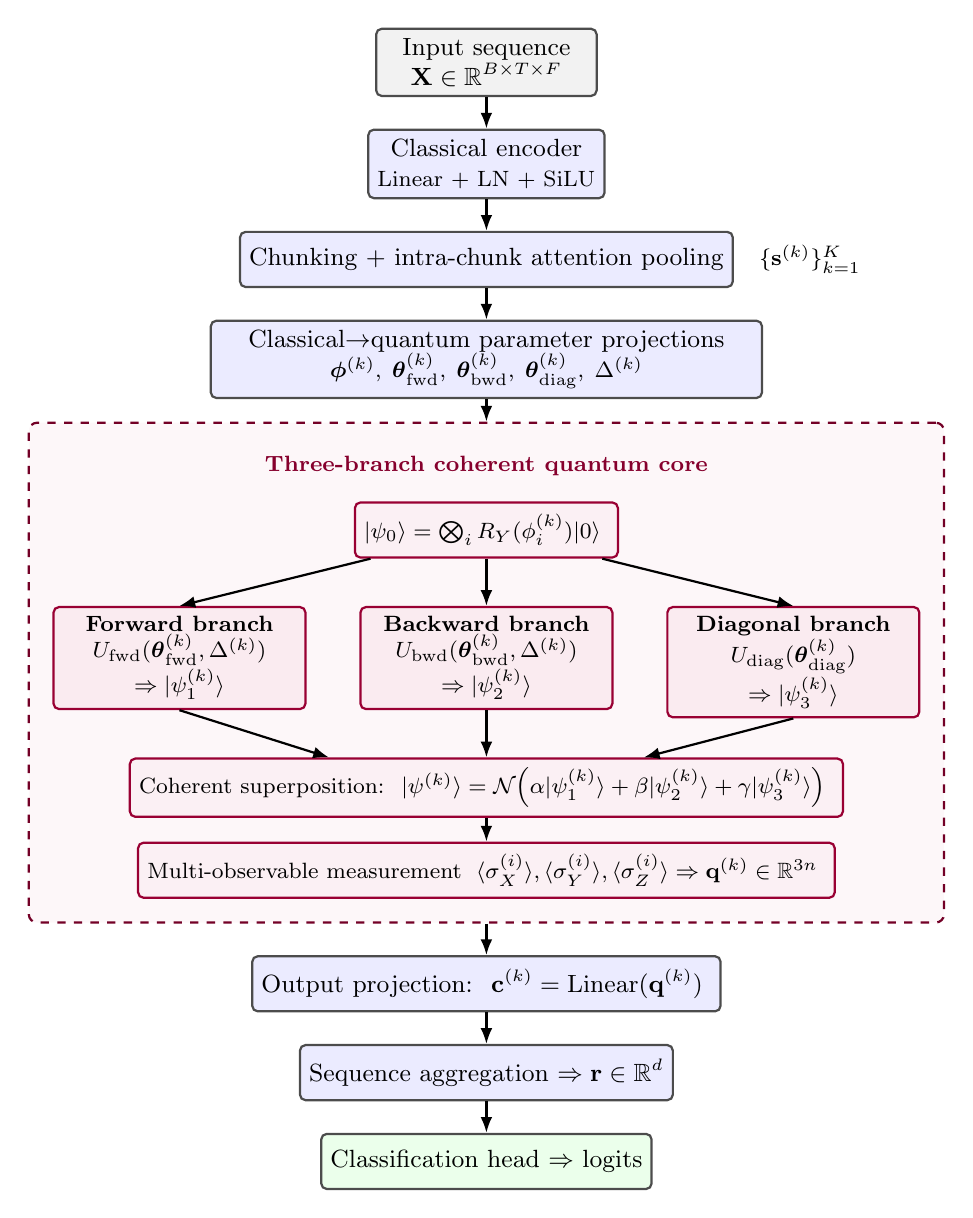
\begin{tikzpicture}[
    font=\small,
    node distance=4mm and 6mm,
    >=Latex,
    classical/.style={
        rectangle, rounded corners=2pt,
        draw=black!70, thick,
        fill=blue!8,
        minimum width=28mm, minimum height=7mm,
        align=center
    },
    cbranch/.style={
        rectangle, rounded corners=2pt,
        draw=black!70, thick,
        fill=blue!8,
        minimum width=22mm, minimum height=6mm,
        align=center, font=\footnotesize
    },
    qbranch/.style={
        rectangle, rounded corners=2pt,
        draw=purple!80!black, thick,
        fill=purple!8,
        minimum width=32mm, minimum height=9mm,
        align=center, font=\footnotesize
    },
    qcore/.style={
        rectangle, rounded corners=2pt,
        draw=purple!80!black, thick,
        fill=purple!6,
        minimum width=28mm, minimum height=7mm,
        align=center, font=\footnotesize
    },
    tensor/.style={font=\footnotesize\itshape},
    arrow/.style={-{Latex[length=2mm]}, thick},
]

% ---------- Input ----------
\node[classical, fill=gray!10] (input) {Input sequence\\$\mathbf{X} \in \mathbb{R}^{B \times T \times F}$};

% ---------- Classical encoder ----------
\node[classical, below=of input] (encoder) {Classical encoder\\\footnotesize Linear $+$ LN $+$ SiLU};

% ---------- Chunking ----------
\node[classical, below=of encoder] (chunk) {Chunking $+$ intra-chunk attention pooling};
\node[tensor, right=2mm of chunk] {$\{\mathbf{s}^{(k)}\}_{k=1}^{K}$};

% ---------- C→Q projections ----------
\node[classical, below=of chunk, minimum width=70mm] (proj) {%
    Classical$\to$quantum parameter projections\\%
    \footnotesize $\boldsymbol{\phi}^{(k)},\;\boldsymbol{\theta}_{\text{fwd}}^{(k)},\;\boldsymbol{\theta}_{\text{bwd}}^{(k)},\;\boldsymbol{\theta}_{\text{diag}}^{(k)},\;\Delta^{(k)}$
};

% ---------- Quantum core (big box) ----------
% Title above the branches
\node[below=6mm of proj, font=\footnotesize\bfseries, text=purple!70!black] (coretitle)
    {Three-branch coherent quantum core};

% Input encoding
\node[qcore, below=2mm of coretitle] (enc) {%
    $|\psi_0\rangle = \bigotimes_i R_Y(\phi_i^{(k)})|0\rangle$
};

% Three branches side by side
\node[qbranch, below left=6mm and 6mm of enc] (fwd) {%
    \textbf{Forward branch}\\%
    $U_{\text{fwd}}(\boldsymbol{\theta}_{\text{fwd}}^{(k)},\Delta^{(k)})$\\%
    $\Rightarrow |\psi_1^{(k)}\rangle$
};
\node[qbranch, below=6mm of enc] (bwd) {%
    \textbf{Backward branch}\\%
    $U_{\text{bwd}}(\boldsymbol{\theta}_{\text{bwd}}^{(k)},\Delta^{(k)})$\\%
    $\Rightarrow |\psi_2^{(k)}\rangle$
};
\node[qbranch, below right=6mm and 6mm of enc] (diag) {%
    \textbf{Diagonal branch}\\%
    $U_{\text{diag}}(\boldsymbol{\theta}_{\text{diag}}^{(k)})$\\%
    $\Rightarrow |\psi_3^{(k)}\rangle$
};

% Coherent superposition
\node[qcore, below=6mm of bwd, minimum width=75mm] (super) {%
    Coherent superposition:\; $|\psi^{(k)}\rangle = \mathcal{N}\!\left(\alpha|\psi_1^{(k)}\rangle + \beta|\psi_2^{(k)}\rangle + \gamma|\psi_3^{(k)}\rangle\right)$
};

% Measurement
\node[qcore, below=3mm of super, minimum width=75mm] (meas) {%
    Multi-observable measurement\; $\langle\sigma_X^{(i)}\rangle,\langle\sigma_Y^{(i)}\rangle,\langle\sigma_Z^{(i)}\rangle \Rightarrow \mathbf{q}^{(k)} \in \mathbb{R}^{3n}$
};

% Bounding box for the core
\begin{pgfonlayer}{background}
\node[
    draw=purple!60!black, thick, dashed, rounded corners=3pt,
    fill=purple!3,
    fit=(coretitle)(enc)(fwd)(diag)(super)(meas),
    inner sep=3mm
] (qcoreBox) {};
\end{pgfonlayer}

% ---------- Output projection ----------
\node[classical, below=4mm of qcoreBox] (outproj) {%
    Output projection:\; $\mathbf{c}^{(k)} = \mathrm{Linear}(\mathbf{q}^{(k)})$
};

% ---------- Sequence aggregation ----------
\node[classical, below=of outproj] (seqagg) {Sequence aggregation $\Rightarrow \mathbf{r} \in \mathbb{R}^{d}$};

% ---------- Classifier ----------
\node[classical, below=of seqagg, fill=green!8] (cls) {Classification head $\Rightarrow$ logits};

% ---------- Arrows ----------
\draw[arrow] (input) -- (encoder);
\draw[arrow] (encoder) -- (chunk);
\draw[arrow] (chunk) -- (proj);
\draw[arrow] (proj) -- (qcoreBox.north);

\draw[arrow] (enc) -- (fwd.north);
\draw[arrow] (enc) -- (bwd);
\draw[arrow] (enc) -- (diag.north);

\draw[arrow] (fwd.south) -- ([xshift=-20mm]super.north);
\draw[arrow] (bwd.south) -- (super.north);
\draw[arrow] (diag.south) -- ([xshift=20mm]super.north);

\draw[arrow] (super) -- (meas);
\draw[arrow] (qcoreBox.south) -- (outproj);
\draw[arrow] (outproj) -- (seqagg);
\draw[arrow] (seqagg) -- (cls);

\end{tikzpicture}
\caption{%
\textbf{Quantum Mamba architecture.}
A classical encoder projects the input sequence $\mathbf{X}$ and partitions it into chunks, each summarized by intra-chunk attention pooling.
For each chunk, the summary $\mathbf{s}^{(k)}$ is mapped through separate linear projections to the quantum input angles $\boldsymbol{\phi}^{(k)}$, three sets of variational parameters $\{\boldsymbol{\theta}_{\text{fwd}}^{(k)}, \boldsymbol{\theta}_{\text{bwd}}^{(k)}, \boldsymbol{\theta}_{\text{diag}}^{(k)}\}$, and a scalar selective-gating factor $\Delta^{(k)}$.
Three independent quantum branches (forward and backward Delta-modulated, diagonal unmodulated) are evolved from the same input state $|\psi_0\rangle$ and coherently combined at the amplitude level through learnable complex coefficients $\alpha, \beta, \gamma$ before multi-observable measurement.
The resulting chunk-level quantum feature vectors $\mathbf{q}^{(k)}$ are then projected back to the model hidden space, aggregated across chunks, and passed through a classification head.%
}
\label{fig:qmamba_architecture}
\end{figure*}

% ============================================================

\begin{figure*}[t]
\centering
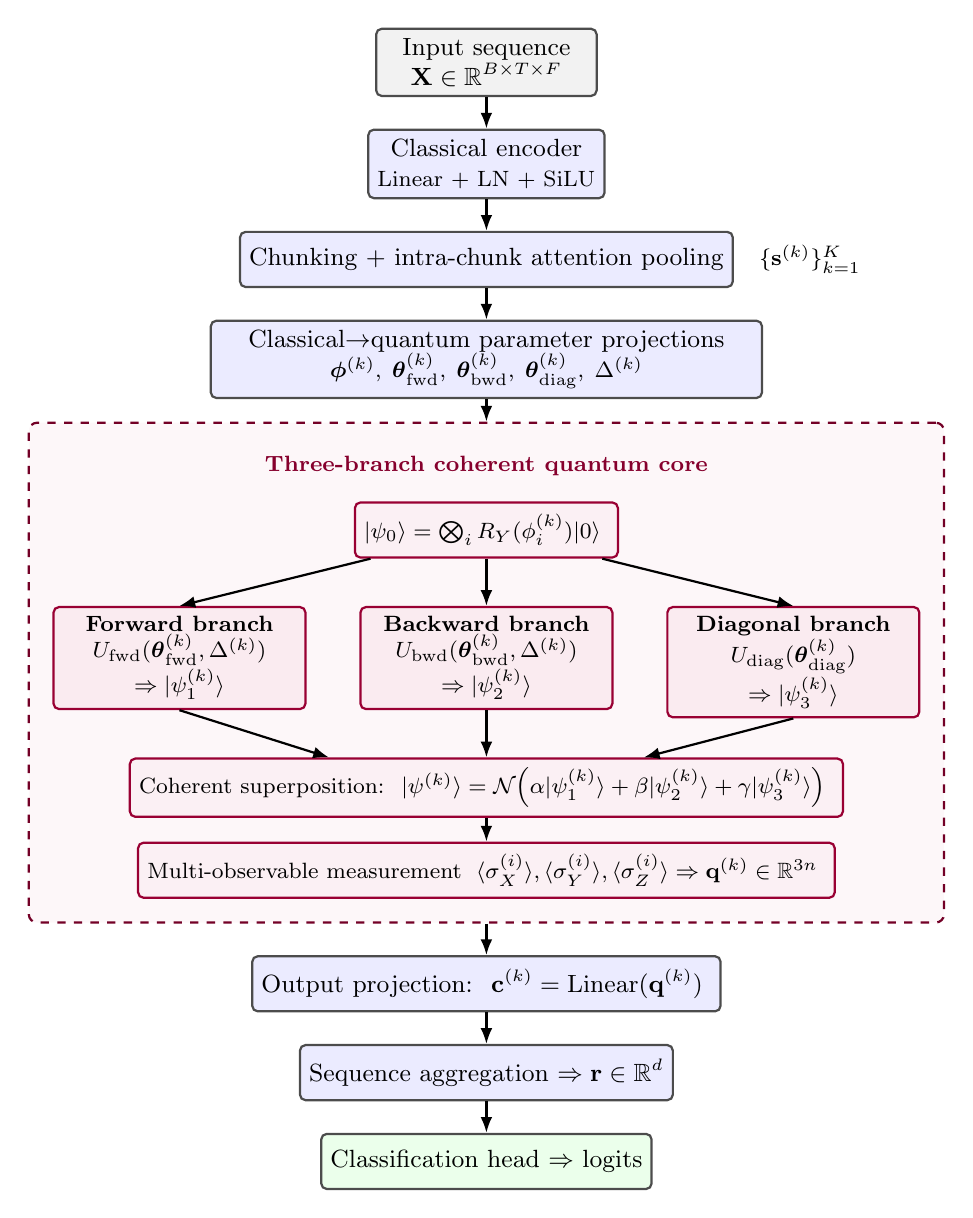
\begin{tikzpicture}[
    font=\small,
    node distance=4mm and 6mm,
    >=Latex,
    classical/.style={
        rectangle, rounded corners=2pt,
        draw=black!70, thick,
        fill=blue!8,
        minimum width=28mm, minimum height=7mm,
        align=center
    },
    cbranch/.style={
        rectangle, rounded corners=2pt,
        draw=black!70, thick,
        fill=blue!8,
        minimum width=22mm, minimum height=6mm,
        align=center, font=\footnotesize
    },
    qbranch/.style={
        rectangle, rounded corners=2pt,
        draw=purple!80!black, thick,
        fill=purple!8,
        minimum width=32mm, minimum height=9mm,
        align=center, font=\footnotesize
    },
    qcore/.style={
        rectangle, rounded corners=2pt,
        draw=purple!80!black, thick,
        fill=purple!6,
        minimum width=28mm, minimum height=7mm,
        align=center, font=\footnotesize
    },
    tensor/.style={font=\footnotesize\itshape},
    arrow/.style={-{Latex[length=2mm]}, thick},
]

% ---------- Input ----------
\node[classical, fill=gray!10] (input) {Input sequence\\$\mathbf{X} \in \mathbb{R}^{B \times T \times F}$};

% ---------- Classical encoder ----------
\node[classical, below=of input] (encoder) {Classical encoder\\\footnotesize Linear $+$ LN $+$ SiLU};

% ---------- Chunking ----------
\node[classical, below=of encoder] (chunk) {Chunking $+$ intra-chunk attention pooling};
\node[tensor, right=2mm of chunk] {$\{\mathbf{s}^{(k)}\}_{k=1}^{K}$};

% ---------- C→Q projections ----------
\node[classical, below=of chunk, minimum width=70mm] (proj) {%
    Classical$\to$quantum parameter projections\\%
    \footnotesize $\boldsymbol{\phi}^{(k)},\;\boldsymbol{\theta}_{\text{fwd}}^{(k)},\;\boldsymbol{\theta}_{\text{bwd}}^{(k)},\;\boldsymbol{\theta}_{\text{diag}}^{(k)},\;\Delta^{(k)}$
};

% ---------- Quantum core (big box) ----------
% Title above the branches
\node[below=6mm of proj, font=\footnotesize\bfseries, text=purple!70!black] (coretitle)
    {Three-branch coherent quantum core};

% Input encoding
\node[qcore, below=2mm of coretitle] (enc) {%
    $|\psi_0\rangle = \bigotimes_i R_Y(\phi_i^{(k)})|0\rangle$
};

% Three branches side by side
\node[qbranch, below left=6mm and 6mm of enc] (fwd) {%
    \textbf{Forward branch}\\%
    $U_{\text{fwd}}(\boldsymbol{\theta}_{\text{fwd}}^{(k)},\Delta^{(k)})$\\%
    $\Rightarrow |\psi_1^{(k)}\rangle$
};
\node[qbranch, below=6mm of enc] (bwd) {%
    \textbf{Backward branch}\\%
    $U_{\text{bwd}}(\boldsymbol{\theta}_{\text{bwd}}^{(k)},\Delta^{(k)})$\\%
    $\Rightarrow |\psi_2^{(k)}\rangle$
};
\node[qbranch, below right=6mm and 6mm of enc] (diag) {%
    \textbf{Diagonal branch}\\%
    $U_{\text{diag}}(\boldsymbol{\theta}_{\text{diag}}^{(k)})$\\%
    $\Rightarrow |\psi_3^{(k)}\rangle$
};

% Coherent superposition
\node[qcore, below=6mm of bwd, minimum width=75mm] (super) {%
    Coherent superposition:\; $|\psi^{(k)}\rangle = \mathcal{N}\!\left(\alpha|\psi_1^{(k)}\rangle + \beta|\psi_2^{(k)}\rangle + \gamma|\psi_3^{(k)}\rangle\right)$
};

% Measurement
\node[qcore, below=3mm of super, minimum width=75mm] (meas) {%
    Multi-observable measurement\; $\langle\sigma_X^{(i)}\rangle,\langle\sigma_Y^{(i)}\rangle,\langle\sigma_Z^{(i)}\rangle \Rightarrow \mathbf{q}^{(k)} \in \mathbb{R}^{3n}$
};

% Bounding box for the core
\begin{pgfonlayer}{background}
\node[
    draw=purple!60!black, thick, dashed, rounded corners=3pt,
    fill=purple!3,
    fit=(coretitle)(enc)(fwd)(diag)(super)(meas),
    inner sep=3mm
] (qcoreBox) {};
\end{pgfonlayer}

% ---------- Output projection ----------
\node[classical, below=4mm of qcoreBox] (outproj) {%
    Output projection:\; $\mathbf{c}^{(k)} = \mathrm{Linear}(\mathbf{q}^{(k)})$
};

% ---------- Sequence aggregation ----------
\node[classical, below=of outproj] (seqagg) {Sequence aggregation $\Rightarrow \mathbf{r} \in \mathbb{R}^{d}$};

% ---------- Classifier ----------
\node[classical, below=of seqagg, fill=green!8] (cls) {Classification head $\Rightarrow$ logits};

% ---------- Arrows ----------
\draw[arrow] (input) -- (encoder);
\draw[arrow] (encoder) -- (chunk);
\draw[arrow] (chunk) -- (proj);
\draw[arrow] (proj) -- (qcoreBox.north);

\draw[arrow] (enc) -- (fwd.north);
\draw[arrow] (enc) -- (bwd);
\draw[arrow] (enc) -- (diag.north);

\draw[arrow] (fwd.south) -- ([xshift=-20mm]super.north);
\draw[arrow] (bwd.south) -- (super.north);
\draw[arrow] (diag.south) -- ([xshift=20mm]super.north);

\draw[arrow] (super) -- (meas);
\draw[arrow] (qcoreBox.south) -- (outproj);
\draw[arrow] (outproj) -- (seqagg);
\draw[arrow] (seqagg) -- (cls);

\end{tikzpicture}
\caption{%
\textbf{Quantum Mamba architecture.}
A classical encoder projects the input sequence $\mathbf{X}$ and partitions it into chunks, each summarized by intra-chunk attention pooling.
For each chunk, the summary $\mathbf{s}^{(k)}$ is mapped through separate linear projections to the quantum input angles $\boldsymbol{\phi}^{(k)}$, three sets of variational parameters $\{\boldsymbol{\theta}_{\text{fwd}}^{(k)}, \boldsymbol{\theta}_{\text{bwd}}^{(k)}, \boldsymbol{\theta}_{\text{diag}}^{(k)}\}$, and a scalar selective-gating factor $\Delta^{(k)}$.
Three independent quantum branches (forward and backward Delta-modulated, diagonal unmodulated) are evolved from the same input state $|\psi_0\rangle$ and coherently combined at the amplitude level through learnable complex coefficients $\alpha, \beta, \gamma$ before multi-observable measurement.
The resulting chunk-level quantum feature vectors $\mathbf{q}^{(k)}$ are then projected back to the model hidden space, aggregated across chunks, and passed through a classification head.%
}
\label{fig:qmamba_architecture}
\end{figure*}


\subsubsection{Classical encoder and chunking}
The input is first projected into the model hidden space via a linear layer followed by layer normalization, SiLU activation, and dropout:
\begin{equation}
    \mathbf{H} = \mathrm{Encoder}(\mathbf{X}) \in \mathbb{R}^{B \times T \times d}.
    \label{eq:input_proj}
\end{equation}
To interface the variable-length sequence with the fixed-width quantum circuit, $\mathbf{H}$ is partitioned into $K = \lceil T/C \rceil$ non-overlapping chunks (zero-padding the last chunk if needed), and each chunk is summarized by a learned attention-pooled vector:
\begin{equation}
    \mathbf{s}^{(k)} = \sum_{t=1}^{C} \alpha_t^{(k)}\, \mathbf{h}_t^{(k)},
    \qquad
    \boldsymbol{\alpha}^{(k)} = \mathrm{softmax}\!\big(f_{\mathrm{attn}}(\mathbf{H}^{(k)})\big) \in \mathbb{R}^{C}.
    \label{eq:chunk_summary}
\end{equation}
Each summary $\mathbf{s}^{(k)} \in \mathbb{R}^{d}$ is then transformed into a complete set of classical-to-quantum interface parameters by four linear projections: an $n$-dimensional input-angle vector
\begin{equation}
    \boldsymbol{\phi}^{(k)} = \pi\cdot\tanh\!\big(\mathbf{W}_{\text{enc}}\,\mathbf{s}^{(k)} + \mathbf{b}_{\text{enc}}\big) \in [-\pi, \pi]^{n},
    \label{eq:input_angles}
\end{equation}
three variational parameter vectors $\boldsymbol{\theta}_{\text{fwd}}^{(k)}, \boldsymbol{\theta}_{\text{bwd}}^{(k)}, \boldsymbol{\theta}_{\text{diag}}^{(k)} \in \mathbb{R}^{5nL}$ (one per quantum branch), and a scalar Mamba-style selective gating factor
\begin{equation}
    \Delta^{(k)} = \sigma\!\big(f_{\Delta}(\mathbf{s}^{(k)})\big) \in [0, 1].
    \label{eq:delta}
\end{equation}

\subsubsection{Three-branch coherent quantum core}
\label{sec:qm_core}
The quantum core is the central contribution of our architecture. Rather than processing each chunk through a single parameterized circuit, we evolve \emph{three independent quantum branches}---a forward branch, a backward branch, and a diagonal branch---and combine their state vectors coherently (at the amplitude level) \emph{before} measurement.

Each branch begins by encoding the input angles $\boldsymbol{\phi}^{(k)}$ via single-qubit $R_Y$ rotations, $|\psi_0\rangle = \bigotimes_{i=0}^{n-1} R_Y(\phi_i^{(k)})|0\rangle$, and then applies $L$ variational layers.
A single layer consists of arbitrary single-qubit rotations $R_X R_Y R_Z$ on each qubit followed by two controlled-$R_X$ entangling rings (one in the forward direction $i \to i{+}1$, one in the backward direction $i \to i{-}1$, both with periodic boundary), for a total of $5n$ trainable parameters per layer.
The three branches share this ansatz structure but differ in how they use the Delta factor and in the spatial ordering of their gates:
\begin{itemize}
    \item \textbf{Forward branch} $|\psi_1^{(k)}\rangle$: applies $U_{\text{fwd}}(\boldsymbol{\theta}_{\text{fwd}}^{(k)}, \Delta^{(k)})$, in which every single-qubit rotation angle is multiplied by $\Delta^{(k)}$. The entangling CRX gates are left unmodulated, preserving the entanglement topology regardless of the gating level. This mirrors the input-dependent discretization of classical Mamba~\cite{Gu2024}: when $\Delta^{(k)} \to 0$, the branch approaches identity (the chunk is ``forgotten''); when $\Delta^{(k)} \to 1$, the full rotations are applied.
    \item \textbf{Backward branch} $|\psi_2^{(k)}\rangle$: applies $U_{\text{bwd}}(\boldsymbol{\theta}_{\text{bwd}}^{(k)}, \Delta^{(k)})$, which uses the same Delta-modulated structure but traverses the qubit register in reverse order (rotations from qubit $n{-}1$ down to $0$, backward CRX ring before forward CRX ring). This produces an anti-causal state evolution complementary to the forward branch.
    \item \textbf{Diagonal branch} $|\psi_3^{(k)}\rangle$: applies $U_{\text{diag}}(\boldsymbol{\theta}_{\text{diag}}^{(k)})$ using the standard (unmodulated) ansatz. This branch acts as a skip-connection-like pathway that provides a stable, Delta-independent gradient flow and captures features that do not require selective gating.
\end{itemize}

Two design choices distinguish this core from prior quantum sequence models. First, the Delta factor here modulates quantum rotation angles \emph{directly inside the circuit}, in contrast to QMamba~\cite{Stenzel2025}, where Delta acts on the classical SSM matrices; this brings Mamba's input-dependent selective forgetting into the quantum domain. Second, because the core operates on a fixed register of $n$ main qubits per chunk, both the quantum circuit width and depth are independent of the sequence length $T$, keeping the design compatible with near-term hardware constraints.

The three branch states are then combined through learnable complex coefficients $\alpha, \beta, \gamma \in \mathbb{C}$ (initialized to $1/\sqrt{3}$) and renormalized:
\begin{equation}
    |\psi^{(k)}\rangle = \mathcal{N}\!\left(\alpha\,|\psi_1^{(k)}\rangle + \beta\,|\psi_2^{(k)}\rangle + \gamma\,|\psi_3^{(k)}\rangle\right),
    \label{eq:superposition}
\end{equation} %%
where $\mathcal{N}(\cdot)$ denotes normalization to unit length.
This coherent combination is the defining operation of the core: because the branches are summed at the amplitude level \emph{before} measurement, the resulting expectation values include interference cross terms of the form $c_j^{*} c_k \langle\psi_j|\hat{O}|\psi_k\rangle$ for $j \neq k$---a genuinely quantum effect that cannot be replicated by any classical convex combination of the individual branch measurements.

Finally, the combined state is measured using the full Pauli set on each qubit, yielding a $3n$-dimensional quantum feature vector:
\begin{equation}
    \mathbf{q}^{(k)} = \Big(\langle\sigma_X^{(i)}\rangle,\; \langle\sigma_Y^{(i)}\rangle,\; \langle\sigma_Z^{(i)}\rangle\Big)_{i=0}^{n-1} \in \mathbb{R}^{3n},
    \label{eq:measurement}
\end{equation}
where all expectation values are taken with respect to $|\psi^{(k)}\rangle$.
Measuring all three Paulis provides a tomographically richer characterization of the state than $\sigma_Z$ alone, at the cost of additional expectation-value estimation.

\subsubsection{Sequence aggregation and classification}
Each quantum feature $\mathbf{q}^{(k)}$ is projected back into the model hidden space through a linear layer with layer normalization and SiLU activation, yielding chunk-level representations $\mathbf{c}^{(k)} \in \mathbb{R}^{d}$.
A second learned attention mechanism aggregates these chunk representations into a single sequence-level vector $\mathbf{r} \in \mathbb{R}^{d}$ (analogous to Eq.~\eqref{eq:chunk_summary} but operating over chunks instead of timesteps), which is then passed through a two-layer MLP classification head to produce the output logits.

% ============================================================
\subsection{Quantum Hydra}
\label{sec:quantum_hydra}

Quantum Hydra extends Quantum Mamba to process sequences in \emph{both} temporal directions, capturing causal and anti-causal dependencies in a manner inspired by classical bidirectional SSMs~\cite{Hwang}.
It shares the classical encoder, chunking, and classification stages of Quantum Mamba, but replaces the single quantum core with \emph{two} independent three-branch coherent cores: one that processes the chunk sequence in the natural temporal order ($k = 1, \ldots, K$) and one that processes it in reverse.
Fig.~\ref{fig:qhydra_architecture} shows the overall architecture.
% ============================================================
% Quantum Hydra architecture diagram (TikZ)
% Include in main document with:
%   \usepackage{tikz}
%   \usepackage{graphicx}  % for \scalebox
%   \usetikzlibrary{positioning, arrows.meta, fit, backgrounds, calc, shapes.geometric}
%   % ============================================================
% Quantum Hydra architecture diagram (TikZ)
% Include in main document with:
%   \usepackage{tikz}
%   \usepackage{graphicx}  % for \scalebox
%   \usetikzlibrary{positioning, arrows.meta, fit, backgrounds, calc, shapes.geometric}
%   % ============================================================
% Quantum Hydra architecture diagram (TikZ)
% Include in main document with:
%   \usepackage{tikz}
%   \usepackage{graphicx}  % for \scalebox
%   \usetikzlibrary{positioning, arrows.meta, fit, backgrounds, calc, shapes.geometric}
%   \input{fig_quantum_hydra.tex}
% ============================================================

\begin{figure*}[t]
\centering
\scalebox{0.85}{%
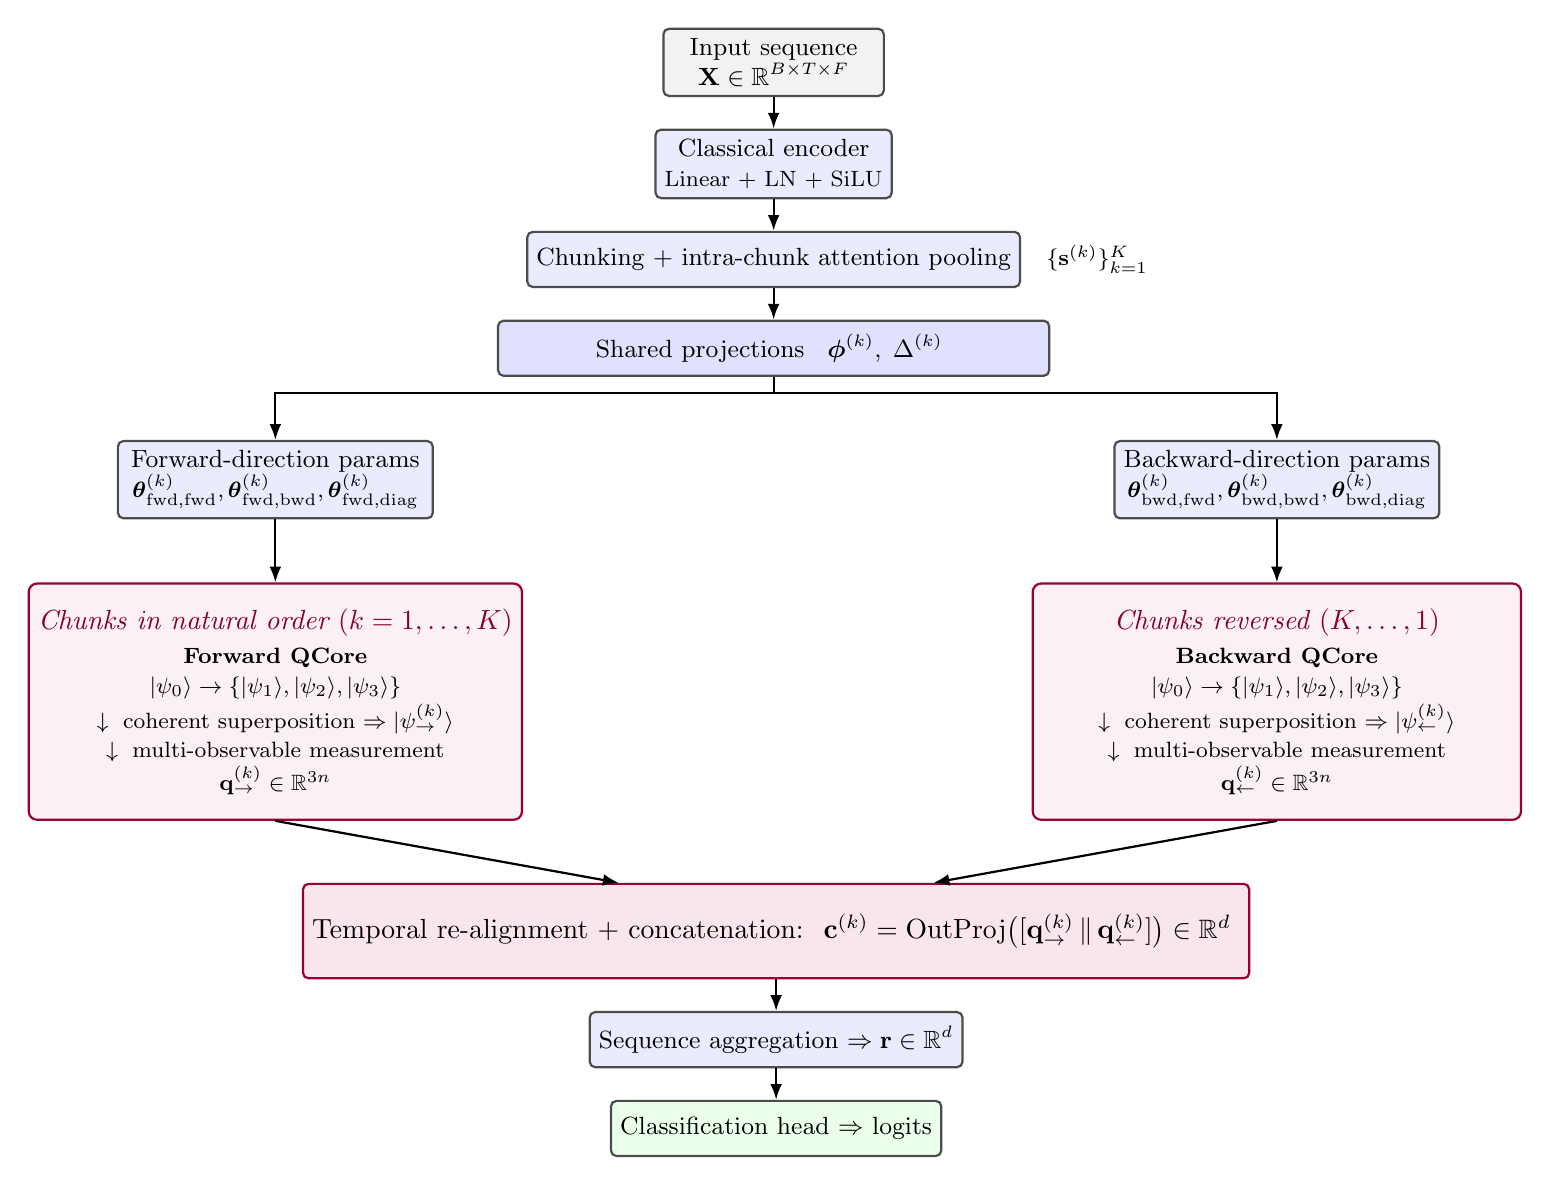
\begin{tikzpicture}[
    font=\small,
    node distance=4mm and 6mm,
    >=Latex,
    classical/.style={
        rectangle, rounded corners=2pt,
        draw=black!70, thick,
        fill=blue!8,
        minimum width=28mm, minimum height=7mm,
        align=center
    },
    qcore/.style={
        rectangle, rounded corners=3pt,
        draw=purple!80!black, thick,
        fill=purple!6,
        minimum width=62mm, minimum height=30mm,
        align=center, font=\footnotesize
    },
    fusion/.style={
        rectangle, rounded corners=2pt,
        draw=purple!80!black, thick,
        fill=purple!10,
        minimum width=96mm, minimum height=12mm,
        align=center, font=\fontsize{9.6pt}{11.5pt}\selectfont
    },
    tensor/.style={font=\footnotesize\itshape},
    arrow/.style={-{Latex[length=2mm]}, thick},
]

% ---------- Input ----------
\node[classical, fill=gray!10] (input) {Input sequence\\$\mathbf{X} \in \mathbb{R}^{B \times T \times F}$};

% ---------- Classical encoder ----------
\node[classical, below=of input] (encoder) {Classical encoder\\\footnotesize Linear $+$ LN $+$ SiLU};

% ---------- Chunking ----------
\node[classical, below=of encoder] (chunk) {Chunking $+$ intra-chunk attention pooling};
\node[tensor, right=2mm of chunk] {$\{\mathbf{s}^{(k)}\}_{k=1}^{K}$};

% ---------- Shared projections (angles + Delta) ----------
\node[classical, below=of chunk, minimum width=70mm, fill=blue!12] (shared) {%
    Shared projections\;\; $\boldsymbol{\phi}^{(k)},\;\Delta^{(k)}$
};

% ---------- Direction-specific projections ----------
\node[classical, below left=8mm and 8mm of shared, minimum width=40mm] (fwdproj) {%
    Forward-direction params\\%
    \footnotesize $\boldsymbol{\theta}_{\text{fwd,fwd}}^{(k)},\boldsymbol{\theta}_{\text{fwd,bwd}}^{(k)},\boldsymbol{\theta}_{\text{fwd,diag}}^{(k)}$
};
\node[classical, below right=8mm and 8mm of shared, minimum width=40mm] (bwdproj) {%
    Backward-direction params\\%
    \footnotesize $\boldsymbol{\theta}_{\text{bwd,fwd}}^{(k)},\boldsymbol{\theta}_{\text{bwd,bwd}}^{(k)},\boldsymbol{\theta}_{\text{bwd,diag}}^{(k)}$
};

% ---------- Two quantum cores (direction labels placed INSIDE) ----------
\node[qcore, below=8mm of fwdproj] (coreF) {%
    \textcolor{purple!70!black}{{\fontsize{9.6pt}{11.5pt}\selectfont\textit{Chunks in natural order $(k=1,\dots,K)$}}}\\[1mm]%
    \textbf{Forward QCore}\\[0.5mm]%
    $|\psi_0\rangle \to \{|\psi_1\rangle,|\psi_2\rangle,|\psi_3\rangle\}$\\[0.3mm]%
    $\downarrow$\; coherent superposition $\Rightarrow |\psi_{\rightarrow}^{(k)}\rangle$\\[0.3mm]%
    $\downarrow$\; multi-observable measurement\\[0.3mm]%
    $\mathbf{q}_{\rightarrow}^{(k)} \in \mathbb{R}^{3n}$
};

\node[qcore, below=8mm of bwdproj] (coreB) {%
    \textcolor{purple!70!black}{{\fontsize{9.6pt}{11.5pt}\selectfont\textit{Chunks reversed $(K,\dots,1)$}}}\\[1mm]%
    \textbf{Backward QCore}\\[0.5mm]%
    $|\psi_0\rangle \to \{|\psi_1\rangle,|\psi_2\rangle,|\psi_3\rangle\}$\\[0.3mm]%
    $\downarrow$\; coherent superposition $\Rightarrow |\psi_{\leftarrow}^{(k)}\rangle$\\[0.3mm]%
    $\downarrow$\; multi-observable measurement\\[0.3mm]%
    $\mathbf{q}_{\leftarrow}^{(k)} \in \mathbb{R}^{3n}$
};

% ---------- Temporal re-alignment + concat (positioned via explicit coordinate) ----------
\node[fusion] (fuse) at ($(coreF.south)!0.5!(coreB.south) + (0,-14mm)$) {%
    Temporal re-alignment $+$ concatenation:\;
    $\mathbf{c}^{(k)} = \mathrm{OutProj}\!\left([\mathbf{q}_{\rightarrow}^{(k)} \,\|\, \mathbf{q}_{\leftarrow}^{(k)}]\right) \in \mathbb{R}^{d}$
};

% ---------- Sequence aggregation ----------
\node[classical, below=of fuse] (seqagg) {Sequence aggregation $\Rightarrow \mathbf{r} \in \mathbb{R}^{d}$};

% ---------- Classifier ----------
\node[classical, below=of seqagg, fill=green!8] (cls) {Classification head $\Rightarrow$ logits};

% ---------- Arrows ----------
\draw[arrow] (input) -- (encoder);
\draw[arrow] (encoder) -- (chunk);
\draw[arrow] (chunk) -- (shared);

% Shared projections feed both cores
\draw[arrow] (shared.south) -- ++(0,-2mm) -| (fwdproj.north);
\draw[arrow] (shared.south) -- ++(0,-2mm) -| (bwdproj.north);

\draw[arrow] (fwdproj) -- (coreF);
\draw[arrow] (bwdproj) -- (coreB);

% Clean diagonal arrows from cores to fuse box (no overlapping L-bends)
\draw[arrow] (coreF.south) -- ([xshift=-20mm]fuse.north);
\draw[arrow] (coreB.south) -- ([xshift=20mm]fuse.north);

\draw[arrow] (fuse) -- (seqagg);
\draw[arrow] (seqagg) -- (cls);

\end{tikzpicture}%
}
\caption{%
\textbf{Quantum Hydra architecture.}
Quantum Hydra extends Quantum Mamba to process sequences in \emph{both} temporal directions.
The classical encoder, chunking, and shared projections for the input angles $\boldsymbol{\phi}^{(k)}$ and selective-gating factor $\Delta^{(k)}$ are identical to Quantum Mamba.
Two independent three-branch coherent quantum cores are used in parallel: the \emph{forward core} processes the chunk-summary sequence in its natural temporal order, while the \emph{backward core} processes the reversed sequence with its own dedicated set of variational parameter projections.
The resulting chunk-level feature vectors are re-aligned in time, concatenated, and projected back to the model hidden space before sequence aggregation and classification.
This design captures both causal and anti-causal temporal dependencies at the cost of roughly $2\times$ the quantum circuit evaluations per chunk compared to Quantum Mamba.%
}
\label{fig:qhydra_architecture}
\end{figure*}

% ============================================================

\begin{figure*}[t]
\centering
\scalebox{0.85}{%
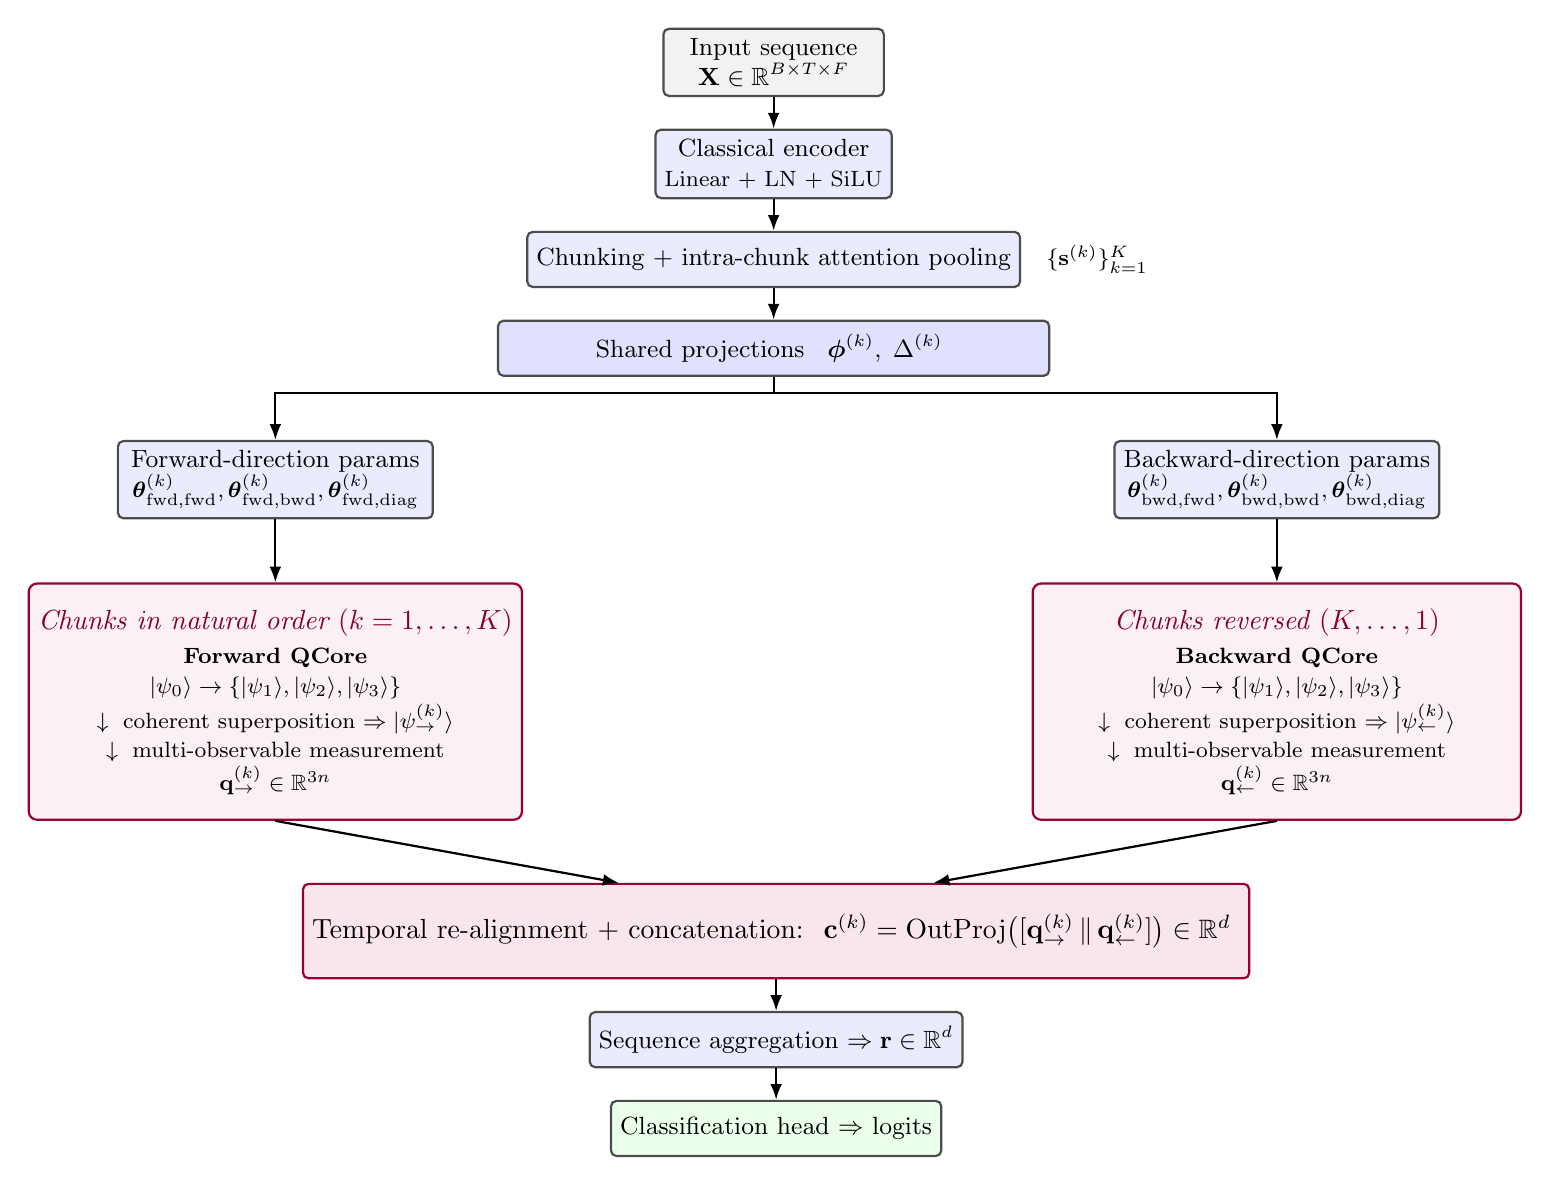
\begin{tikzpicture}[
    font=\small,
    node distance=4mm and 6mm,
    >=Latex,
    classical/.style={
        rectangle, rounded corners=2pt,
        draw=black!70, thick,
        fill=blue!8,
        minimum width=28mm, minimum height=7mm,
        align=center
    },
    qcore/.style={
        rectangle, rounded corners=3pt,
        draw=purple!80!black, thick,
        fill=purple!6,
        minimum width=62mm, minimum height=30mm,
        align=center, font=\footnotesize
    },
    fusion/.style={
        rectangle, rounded corners=2pt,
        draw=purple!80!black, thick,
        fill=purple!10,
        minimum width=96mm, minimum height=12mm,
        align=center, font=\fontsize{9.6pt}{11.5pt}\selectfont
    },
    tensor/.style={font=\footnotesize\itshape},
    arrow/.style={-{Latex[length=2mm]}, thick},
]

% ---------- Input ----------
\node[classical, fill=gray!10] (input) {Input sequence\\$\mathbf{X} \in \mathbb{R}^{B \times T \times F}$};

% ---------- Classical encoder ----------
\node[classical, below=of input] (encoder) {Classical encoder\\\footnotesize Linear $+$ LN $+$ SiLU};

% ---------- Chunking ----------
\node[classical, below=of encoder] (chunk) {Chunking $+$ intra-chunk attention pooling};
\node[tensor, right=2mm of chunk] {$\{\mathbf{s}^{(k)}\}_{k=1}^{K}$};

% ---------- Shared projections (angles + Delta) ----------
\node[classical, below=of chunk, minimum width=70mm, fill=blue!12] (shared) {%
    Shared projections\;\; $\boldsymbol{\phi}^{(k)},\;\Delta^{(k)}$
};

% ---------- Direction-specific projections ----------
\node[classical, below left=8mm and 8mm of shared, minimum width=40mm] (fwdproj) {%
    Forward-direction params\\%
    \footnotesize $\boldsymbol{\theta}_{\text{fwd,fwd}}^{(k)},\boldsymbol{\theta}_{\text{fwd,bwd}}^{(k)},\boldsymbol{\theta}_{\text{fwd,diag}}^{(k)}$
};
\node[classical, below right=8mm and 8mm of shared, minimum width=40mm] (bwdproj) {%
    Backward-direction params\\%
    \footnotesize $\boldsymbol{\theta}_{\text{bwd,fwd}}^{(k)},\boldsymbol{\theta}_{\text{bwd,bwd}}^{(k)},\boldsymbol{\theta}_{\text{bwd,diag}}^{(k)}$
};

% ---------- Two quantum cores (direction labels placed INSIDE) ----------
\node[qcore, below=8mm of fwdproj] (coreF) {%
    \textcolor{purple!70!black}{{\fontsize{9.6pt}{11.5pt}\selectfont\textit{Chunks in natural order $(k=1,\dots,K)$}}}\\[1mm]%
    \textbf{Forward QCore}\\[0.5mm]%
    $|\psi_0\rangle \to \{|\psi_1\rangle,|\psi_2\rangle,|\psi_3\rangle\}$\\[0.3mm]%
    $\downarrow$\; coherent superposition $\Rightarrow |\psi_{\rightarrow}^{(k)}\rangle$\\[0.3mm]%
    $\downarrow$\; multi-observable measurement\\[0.3mm]%
    $\mathbf{q}_{\rightarrow}^{(k)} \in \mathbb{R}^{3n}$
};

\node[qcore, below=8mm of bwdproj] (coreB) {%
    \textcolor{purple!70!black}{{\fontsize{9.6pt}{11.5pt}\selectfont\textit{Chunks reversed $(K,\dots,1)$}}}\\[1mm]%
    \textbf{Backward QCore}\\[0.5mm]%
    $|\psi_0\rangle \to \{|\psi_1\rangle,|\psi_2\rangle,|\psi_3\rangle\}$\\[0.3mm]%
    $\downarrow$\; coherent superposition $\Rightarrow |\psi_{\leftarrow}^{(k)}\rangle$\\[0.3mm]%
    $\downarrow$\; multi-observable measurement\\[0.3mm]%
    $\mathbf{q}_{\leftarrow}^{(k)} \in \mathbb{R}^{3n}$
};

% ---------- Temporal re-alignment + concat (positioned via explicit coordinate) ----------
\node[fusion] (fuse) at ($(coreF.south)!0.5!(coreB.south) + (0,-14mm)$) {%
    Temporal re-alignment $+$ concatenation:\;
    $\mathbf{c}^{(k)} = \mathrm{OutProj}\!\left([\mathbf{q}_{\rightarrow}^{(k)} \,\|\, \mathbf{q}_{\leftarrow}^{(k)}]\right) \in \mathbb{R}^{d}$
};

% ---------- Sequence aggregation ----------
\node[classical, below=of fuse] (seqagg) {Sequence aggregation $\Rightarrow \mathbf{r} \in \mathbb{R}^{d}$};

% ---------- Classifier ----------
\node[classical, below=of seqagg, fill=green!8] (cls) {Classification head $\Rightarrow$ logits};

% ---------- Arrows ----------
\draw[arrow] (input) -- (encoder);
\draw[arrow] (encoder) -- (chunk);
\draw[arrow] (chunk) -- (shared);

% Shared projections feed both cores
\draw[arrow] (shared.south) -- ++(0,-2mm) -| (fwdproj.north);
\draw[arrow] (shared.south) -- ++(0,-2mm) -| (bwdproj.north);

\draw[arrow] (fwdproj) -- (coreF);
\draw[arrow] (bwdproj) -- (coreB);

% Clean diagonal arrows from cores to fuse box (no overlapping L-bends)
\draw[arrow] (coreF.south) -- ([xshift=-20mm]fuse.north);
\draw[arrow] (coreB.south) -- ([xshift=20mm]fuse.north);

\draw[arrow] (fuse) -- (seqagg);
\draw[arrow] (seqagg) -- (cls);

\end{tikzpicture}%
}
\caption{%
\textbf{Quantum Hydra architecture.}
Quantum Hydra extends Quantum Mamba to process sequences in \emph{both} temporal directions.
The classical encoder, chunking, and shared projections for the input angles $\boldsymbol{\phi}^{(k)}$ and selective-gating factor $\Delta^{(k)}$ are identical to Quantum Mamba.
Two independent three-branch coherent quantum cores are used in parallel: the \emph{forward core} processes the chunk-summary sequence in its natural temporal order, while the \emph{backward core} processes the reversed sequence with its own dedicated set of variational parameter projections.
The resulting chunk-level feature vectors are re-aligned in time, concatenated, and projected back to the model hidden space before sequence aggregation and classification.
This design captures both causal and anti-causal temporal dependencies at the cost of roughly $2\times$ the quantum circuit evaluations per chunk compared to Quantum Mamba.%
}
\label{fig:qhydra_architecture}
\end{figure*}

% ============================================================

\begin{figure*}[t]
\centering
\scalebox{0.85}{%
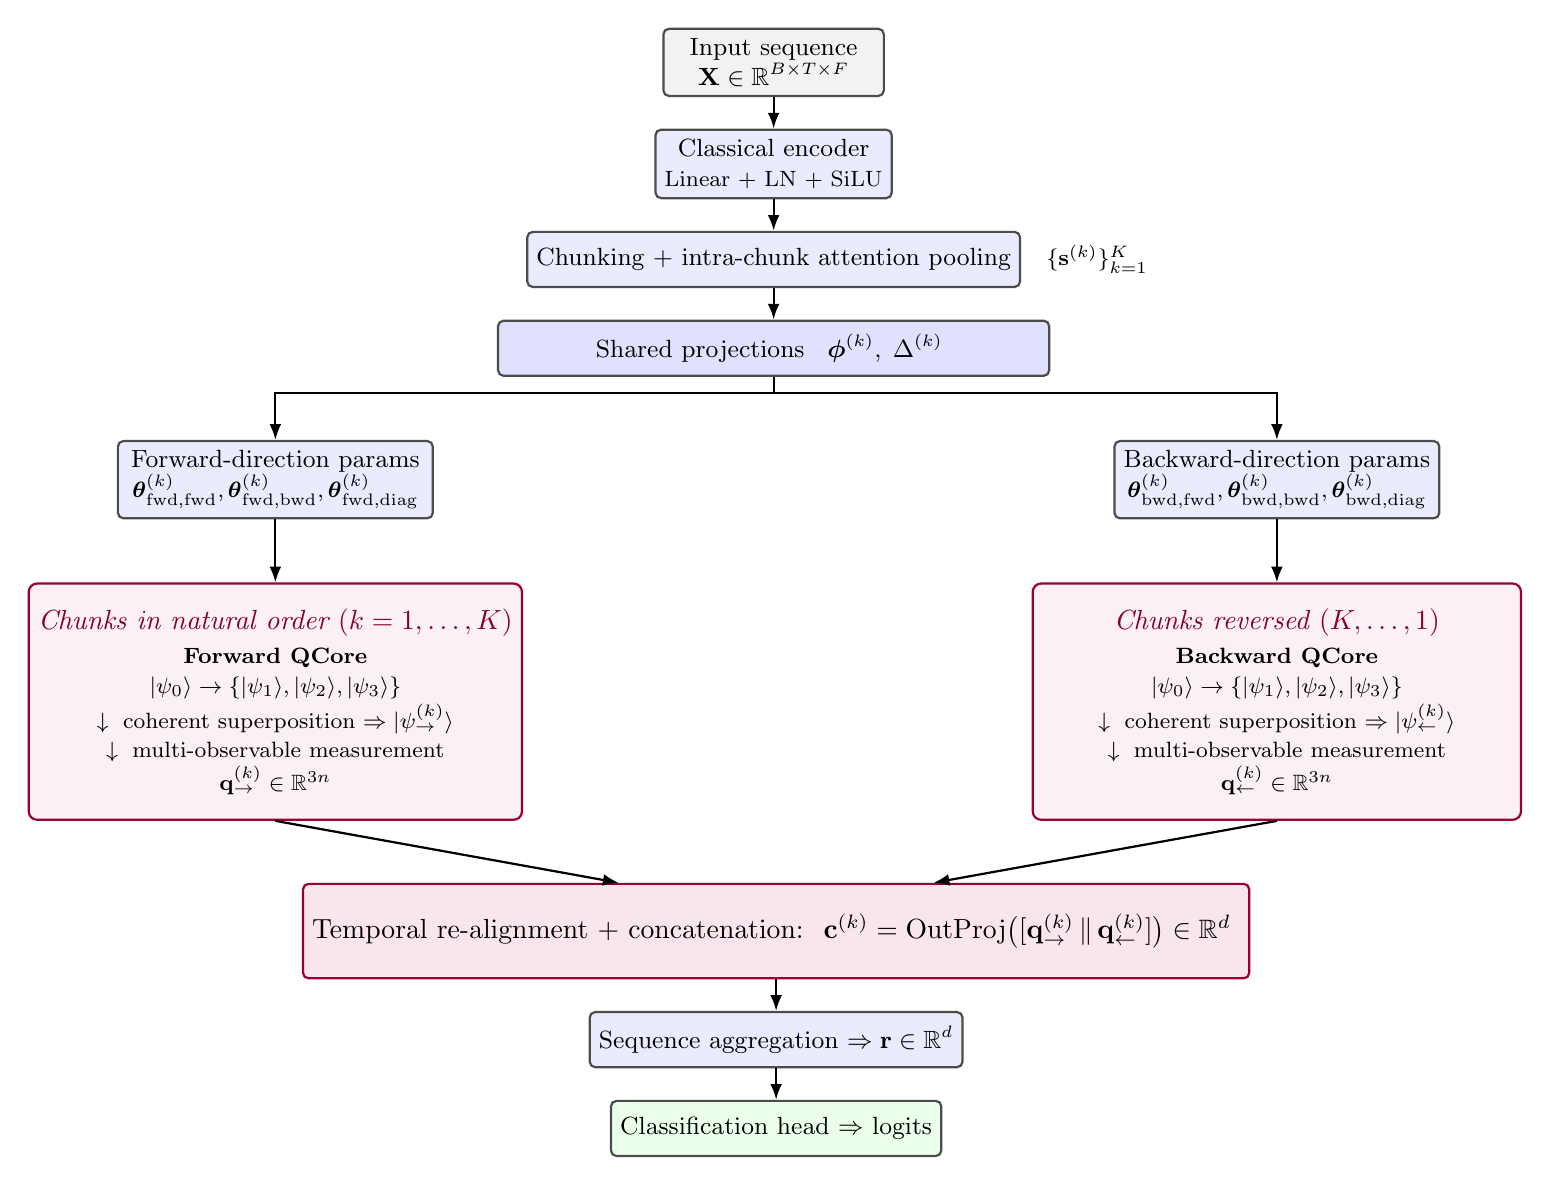
\begin{tikzpicture}[
    font=\small,
    node distance=4mm and 6mm,
    >=Latex,
    classical/.style={
        rectangle, rounded corners=2pt,
        draw=black!70, thick,
        fill=blue!8,
        minimum width=28mm, minimum height=7mm,
        align=center
    },
    qcore/.style={
        rectangle, rounded corners=3pt,
        draw=purple!80!black, thick,
        fill=purple!6,
        minimum width=62mm, minimum height=30mm,
        align=center, font=\footnotesize
    },
    fusion/.style={
        rectangle, rounded corners=2pt,
        draw=purple!80!black, thick,
        fill=purple!10,
        minimum width=96mm, minimum height=12mm,
        align=center, font=\fontsize{9.6pt}{11.5pt}\selectfont
    },
    tensor/.style={font=\footnotesize\itshape},
    arrow/.style={-{Latex[length=2mm]}, thick},
]

% ---------- Input ----------
\node[classical, fill=gray!10] (input) {Input sequence\\$\mathbf{X} \in \mathbb{R}^{B \times T \times F}$};

% ---------- Classical encoder ----------
\node[classical, below=of input] (encoder) {Classical encoder\\\footnotesize Linear $+$ LN $+$ SiLU};

% ---------- Chunking ----------
\node[classical, below=of encoder] (chunk) {Chunking $+$ intra-chunk attention pooling};
\node[tensor, right=2mm of chunk] {$\{\mathbf{s}^{(k)}\}_{k=1}^{K}$};

% ---------- Shared projections (angles + Delta) ----------
\node[classical, below=of chunk, minimum width=70mm, fill=blue!12] (shared) {%
    Shared projections\;\; $\boldsymbol{\phi}^{(k)},\;\Delta^{(k)}$
};

% ---------- Direction-specific projections ----------
\node[classical, below left=8mm and 8mm of shared, minimum width=40mm] (fwdproj) {%
    Forward-direction params\\%
    \footnotesize $\boldsymbol{\theta}_{\text{fwd,fwd}}^{(k)},\boldsymbol{\theta}_{\text{fwd,bwd}}^{(k)},\boldsymbol{\theta}_{\text{fwd,diag}}^{(k)}$
};
\node[classical, below right=8mm and 8mm of shared, minimum width=40mm] (bwdproj) {%
    Backward-direction params\\%
    \footnotesize $\boldsymbol{\theta}_{\text{bwd,fwd}}^{(k)},\boldsymbol{\theta}_{\text{bwd,bwd}}^{(k)},\boldsymbol{\theta}_{\text{bwd,diag}}^{(k)}$
};

% ---------- Two quantum cores (direction labels placed INSIDE) ----------
\node[qcore, below=8mm of fwdproj] (coreF) {%
    \textcolor{purple!70!black}{{\fontsize{9.6pt}{11.5pt}\selectfont\textit{Chunks in natural order $(k=1,\dots,K)$}}}\\[1mm]%
    \textbf{Forward QCore}\\[0.5mm]%
    $|\psi_0\rangle \to \{|\psi_1\rangle,|\psi_2\rangle,|\psi_3\rangle\}$\\[0.3mm]%
    $\downarrow$\; coherent superposition $\Rightarrow |\psi_{\rightarrow}^{(k)}\rangle$\\[0.3mm]%
    $\downarrow$\; multi-observable measurement\\[0.3mm]%
    $\mathbf{q}_{\rightarrow}^{(k)} \in \mathbb{R}^{3n}$
};

\node[qcore, below=8mm of bwdproj] (coreB) {%
    \textcolor{purple!70!black}{{\fontsize{9.6pt}{11.5pt}\selectfont\textit{Chunks reversed $(K,\dots,1)$}}}\\[1mm]%
    \textbf{Backward QCore}\\[0.5mm]%
    $|\psi_0\rangle \to \{|\psi_1\rangle,|\psi_2\rangle,|\psi_3\rangle\}$\\[0.3mm]%
    $\downarrow$\; coherent superposition $\Rightarrow |\psi_{\leftarrow}^{(k)}\rangle$\\[0.3mm]%
    $\downarrow$\; multi-observable measurement\\[0.3mm]%
    $\mathbf{q}_{\leftarrow}^{(k)} \in \mathbb{R}^{3n}$
};

% ---------- Temporal re-alignment + concat (positioned via explicit coordinate) ----------
\node[fusion] (fuse) at ($(coreF.south)!0.5!(coreB.south) + (0,-14mm)$) {%
    Temporal re-alignment $+$ concatenation:\;
    $\mathbf{c}^{(k)} = \mathrm{OutProj}\!\left([\mathbf{q}_{\rightarrow}^{(k)} \,\|\, \mathbf{q}_{\leftarrow}^{(k)}]\right) \in \mathbb{R}^{d}$
};

% ---------- Sequence aggregation ----------
\node[classical, below=of fuse] (seqagg) {Sequence aggregation $\Rightarrow \mathbf{r} \in \mathbb{R}^{d}$};

% ---------- Classifier ----------
\node[classical, below=of seqagg, fill=green!8] (cls) {Classification head $\Rightarrow$ logits};

% ---------- Arrows ----------
\draw[arrow] (input) -- (encoder);
\draw[arrow] (encoder) -- (chunk);
\draw[arrow] (chunk) -- (shared);

% Shared projections feed both cores
\draw[arrow] (shared.south) -- ++(0,-2mm) -| (fwdproj.north);
\draw[arrow] (shared.south) -- ++(0,-2mm) -| (bwdproj.north);

\draw[arrow] (fwdproj) -- (coreF);
\draw[arrow] (bwdproj) -- (coreB);

% Clean diagonal arrows from cores to fuse box (no overlapping L-bends)
\draw[arrow] (coreF.south) -- ([xshift=-20mm]fuse.north);
\draw[arrow] (coreB.south) -- ([xshift=20mm]fuse.north);

\draw[arrow] (fuse) -- (seqagg);
\draw[arrow] (seqagg) -- (cls);

\end{tikzpicture}%
}
\caption{%
\textbf{Quantum Hydra architecture.}
Quantum Hydra extends Quantum Mamba to process sequences in \emph{both} temporal directions.
The classical encoder, chunking, and shared projections for the input angles $\boldsymbol{\phi}^{(k)}$ and selective-gating factor $\Delta^{(k)}$ are identical to Quantum Mamba.
Two independent three-branch coherent quantum cores are used in parallel: the \emph{forward core} processes the chunk-summary sequence in its natural temporal order, while the \emph{backward core} processes the reversed sequence with its own dedicated set of variational parameter projections.
The resulting chunk-level feature vectors are re-aligned in time, concatenated, and projected back to the model hidden space before sequence aggregation and classification.
This design captures both causal and anti-causal temporal dependencies at the cost of roughly $2\times$ the quantum circuit evaluations per chunk compared to Quantum Mamba.%
}
\label{fig:qhydra_architecture}
\end{figure*}
 

Each direction uses its own set of branch parameter projections, so the backward core does not merely reuse the forward parameters.
The backward pass is implemented by reversing the chunk-summary sequence, feeding it through the backward quantum core, and then re-aligning the resulting quantum features with the original temporal order.
Crucially, the input-angle projection and Delta projection layers are \emph{shared} between the two directions, which preserves a consistent data encoding while allowing the direction-specific circuit parameters to specialize.

The forward and backward quantum feature vectors for each chunk are concatenated and projected back to the hidden dimension:
\begin{equation}
    \mathbf{c}^{(k)} = \mathrm{OutProj}\!\Big([\,\mathbf{q}_{\rightarrow}^{(k)} \;\|\; \mathbf{q}_{\leftarrow}^{(k)}\,]\Big) \in \mathbb{R}^{d},
    \label{eq:bidir_fusion}
\end{equation}
where $\|$ denotes concatenation and $\mathrm{OutProj}: \mathbb{R}^{6n} \to \mathbb{R}^{d}$ is a linear layer with layer normalization and SiLU activation.
Sequence aggregation and classification then proceed identically to Quantum Mamba.

Quantum Hydra roughly doubles both the number of quantum circuit evaluations per chunk (from 3 to 6) and the number of classical-to-quantum parameter projections (from 3 to 6), resulting in approximately $2\times$ the training time of Quantum Mamba for the same configuration.
In exchange, it can model bidirectional temporal context within a single-layer quantum core.

% ============================================================
\subsection{Coherent combination vs.\ classical mixing}
\label{sec:rationale}

A natural classical alternative to our three-branch core would be to measure each branch separately and combine the resulting feature vectors, e.g., $\bar{\mathbf{q}} = |\alpha|^2 \mathbf{q}_1 + |\beta|^2 \mathbf{q}_2 + |\gamma|^2 \mathbf{q}_3$.
Such a classical mixture corresponds to the incoherent density operator $\rho_{\text{mix}} = \sum_j |c_j|^2 |\psi_j\rangle\langle\psi_j|$ and retains only the diagonal terms of the combined state, discarding all inter-branch coherence.
In contrast, the expectation value of an observable $\hat{O}$ on the coherently superposed state in Eq.~\eqref{eq:superposition} is
\begin{equation}
    \langle\hat{O}\rangle_{\psi} = \sum_{j} |c_j|^2\, \langle\psi_j|\hat{O}|\psi_j\rangle + \sum_{j \neq k} c_j^{*} c_k\, \langle\psi_j|\hat{O}|\psi_k\rangle,
    \label{eq:interference}
\end{equation}
where $(c_1, c_2, c_3) = (\alpha, \beta, \gamma)$.
The second sum contains the quantum interference cross terms $\langle\psi_j|\hat{O}|\psi_k\rangle$, which encode correlations between the forward, backward, and diagonal processing pathways and are genuinely inaccessible to any classical combination of the individual branch measurements.
By training the coefficients $\alpha, \beta, \gamma$ end-to-end, our models can exploit these interference effects for the downstream task; we hypothesize that this mechanism underlies the empirical quantum-vs-classical gaps reported in our experiments.


\section{Experiments}
\label{sec:experiments}

We evaluate Quantum Mamba and Quantum Hydra on two complementary domains: biomedical time-series classification using two EEG datasets, and natural language understanding using two tasks from the GLUE benchmark.
This pairing tests the same architecture on data with very different statistical properties (continuous multi-channel physiological signals vs.\ discrete tokenized text) and time scales, providing a broad assessment of the proposed models.
Within each domain, we deliberately contrast tasks: a binary, long-sequence motor imagery benchmark (PhysioNet) against a multi-class, clinical-cohort dementia benchmark (ADFTD); and a low-resource sentence-pair entailment task (RTE) against a data-rich single-sentence sentiment task (SST-2). This design probes how the proposed mixing primitive behaves across both task structure (binary vs.\ multi-class, single-sentence vs.\ pair) and training-data regime (data-scarce vs.\ data-rich).

% ============================================================
\subsection{EEG datasets}
\label{sec:eeg_datasets}

\subsubsection{PhysioNet Motor Imagery}
\label{sec:physionet}

The PhysioNet EEG Motor Movement/Imagery Database~\cite{schalk2004bci2000,goldberger2000physiobank} is a widely used benchmark for brain--computer interface research. It contains EEG recordings from 109 healthy subjects performing motor imagery tasks, acquired with a 64-channel BCI2000 system at 160\,Hz.
Following standard practice, we use the three runs (runs 4, 8, and 12) in which subjects imagine opening and closing either the \emph{left} or \emph{right} fist, yielding a binary classification task over 64 EEG channels.

\paragraph{Preprocessing}
Raw EDF recordings are loaded via MNE-Python~\cite{gramfort2013meg}, resampled to a target frequency $f_s \in \{40, 80, 160\}$\,Hz, and epoched to the interval $[1.0, 4.1]$\,s relative to each cue, producing trials of length $T = \lceil 3.1 f_s \rceil$ samples (e.g., $T = 248$ at 80\,Hz).
Signal amplitudes are scaled to millivolts for numerical stability.
Each trial is labeled as left-hand (class 0) or right-hand (class 1) motor imagery.

\paragraph{Baselines and Experimental Setup}
% 여기를 추가

\paragraph{Splits}
To assess cross-subject generalization, we perform a \emph{subject-level} stratified split: 70\% of subjects are assigned to the training set, 15\% to validation, and 15\% to test, ensuring no subject appears in more than one split.

\paragraph{Sampling-frequency ablation.}
We train and evaluate each model at $f_s = 40$, $80$, and $160$\,Hz in order to study how quantum advantage scales with temporal resolution and sequence length.
This yields three sequence lengths ($T = 124, 248, 496$) with identical content but different quantum circuit context windows, allowing us to isolate the effect of sequence length from confounding factors.

\subsubsection{ADFTD Dementia EEG}
\label{sec:adftd}

The ADFTD dataset~\cite{miltiadous2023dataset} is a publicly available resting-state, eyes-closed EEG corpus collected at the 2nd Department of Neurology of AHEPA General Hospital (Thessaloniki, Greece) for the study of dementia.
It contains recordings from 88 subjects: 36 with Alzheimer's disease (AD), 23 with frontotemporal dementia (FTD), and 29 healthy controls (CN).
Data were acquired with a Nihon Kohden EEG 2100 clinical device using 19 scalp electrodes placed according to the international 10--20 system (Fp1, Fp2, F3, F4, C3, C4, P3, P4, O1, O2, F7, F8, T3, T4, T5, T6, Fz, Cz, Pz) at a sampling rate of 500\,Hz.
Recording duration varied from 5 to 21 minutes per subject.
We use the pre-processed version released with the dataset, which has already been (i)~band-pass filtered (0.5--45\,Hz, Butterworth), (ii)~re-referenced to A1--A2, (iii)~artifact-corrected using the Artifact Subspace Reconstruction algorithm, and (iv)~cleaned with ICA-based removal of eye and jaw components via ICLabel.

\paragraph{Preprocessing}
For each subject, we load the .set file using MNE-Python and convert the signal to microvolts.
The continuous recording is then partitioned into non-overlapping fixed-length segments of 2{,}500 samples (5\,seconds at 500\,Hz).
This segmentation yields a consistent trial length across subjects and provides enough per-subject data for batch-level training.
We apply per-channel z-score normalization using statistics computed only from the training set, and clip values to $\pm 10\sigma$ to suppress residual outliers.
Each segment inherits the diagnostic label of its source subject.

\paragraph{Task setup and splits}
We consider the three-class classification task (AD vs.\ FTD vs.\ CN) over the 19-channel $\times$ 2{,}500-sample trials.
As with PhysioNet, we use a \emph{subject-level} stratified split (70\% train / 15\% val / 15\% test) to prevent leakage of subject-specific features between splits, and we stratify by diagnostic group so that the class distribution is preserved across splits.

% ============================================================
\subsection{GLUE benchmark}
\label{sec:glue}

The General Language Understanding Evaluation (GLUE) benchmark~\cite{Wang2018GLUE} is a standard suite of nine English-language natural language understanding tasks used to evaluate the transferability and robustness of sentence-level models.
From this suite, we select two contrasting tasks---SST-2 and RTE---that together stress both abundant-data single-sentence modeling and data-scarce sentence-pair reasoning.

\subsubsection{SST-2: Stanford Sentiment Treebank (binary)}
\label{sec:sst2}

SST-2~\cite{socher2013sst} is a binary sentiment classification task built from movie reviews from Rotten Tomatoes.
Each example is a single sentence labeled as either \emph{positive} or \emph{negative}.
The GLUE release provides approximately 67{,}000 training examples and 872 validation examples, making it by far the largest of the two GLUE tasks we consider and a natural testbed for the models' raw classification capacity.

\subsubsection{RTE: Recognizing Textual Entailment (binary)}
\label{sec:rte}

RTE~\cite{dagan2005pascal,bentivogli2009fifth} is a sentence-pair entailment task aggregated from a series of textual entailment challenges.
Each example consists of a \emph{premise} and a \emph{hypothesis}, and the model must predict whether the premise \emph{entails} the hypothesis (label 0) or not (label 1).
The GLUE release provides only 2{,}490 training examples and 277 validation examples, making RTE a data-scarce, low-resource regime that probes generalization from limited supervision---a setting in which inductive biases of the model architecture become especially important.

\subsubsection{Preprocessing and model interface}
\label{sec:glue_preproc}

Both tasks are loaded directly from the HuggingFace \texttt{datasets} library.
Inputs are tokenized with the pre-trained \texttt{bert-base-uncased} WordPiece tokenizer~\cite{devlin2019bert}: SST-2 sentences are passed as single-segment inputs, while RTE premise--hypothesis pairs are joined using the standard \texttt{[CLS]\,premise\,[SEP]\,hypothesis\,[SEP]} format.
All sequences are padded or truncated to a fixed length of $T = 128$ tokens, with an attention mask tracking valid positions.
Token IDs are then passed through a trainable embedding layer of dimension $d$ to produce a continuous sequence $\mathbf{X} \in \mathbb{R}^{B \times 128 \times d}$, which serves as the input to Quantum Mamba or Quantum Hydra in place of the raw feature matrix used for EEG (Eq.~\eqref{eq:input_proj}).
In this setting, the ``channel'' dimension $F$ of our models corresponds to the token embedding dimension, and the chunked temporal processing operates over token positions instead of time steps.

\paragraph{Labels and metrics}
Both SST-2 and RTE are binary classification tasks; we train with standard cross-entropy loss and report accuracy on the GLUE development set, following the common GLUE evaluation protocol since test-set labels are hidden behind an online submission server.

\begin{table*}[t]
\centering
\caption{Validation Performance (Mean $\pm$ Std)}
\label{tab:val_results}
\renewcommand{\arraystretch}{1.2}
\begin{tabular}{ll ccc ccc}
\toprule
& & \multicolumn{3}{c}{Classical} & \multicolumn{3}{c}{Quantum} \\
\cmidrule(lr){3-5} \cmidrule(lr){6-8}
Task & Model & ACC & F1 & AUC & ACC & F1 & AUC \\
\midrule
ADFTD
 & Hydra
   & \textbf{0.544 $\pm$ 0.052} & 0.593 $\pm$ 0.033 & 0.683 $\pm$ 0.039
   & 0.496 $\pm$ 0.035 & 0.541 $\pm$ 0.010 & 0.661 $\pm$ 0.027 \\
 & Mamba
   & 0.533 $\pm$ 0.069 & \textbf{0.594 $\pm$ 0.081} & \textbf{0.700 $\pm$ 0.070}
   & 0.511 $\pm$ 0.088 & 0.550 $\pm$ 0.013 & 0.617 $\pm$ 0.093 \\
 & Transformer
   & 0.491 $\pm$ 0.054 & 0.512 $\pm$ 0.036 & 0.651 $\pm$ 0.060
   & 0.492 $\pm$ 0.116 & 0.530 $\pm$ 0.053  & 0.612 $\pm$ 0.089 \\
\midrule
PhysioNet
 & Hydra
   & 0.615 $\pm$ 0.104 & 0.674 $\pm$ 0.055 & 0.682 $\pm$ 0.157
   & 0.739 $\pm$ 0.041 & --- & 0.806 $\pm$ 0.047 \\
 & Mamba
   & 0.763 $\pm$ 0.027 & 0.754 $\pm$ 0.038 & 0.845 $\pm$ 0.006
   & 0.742 $\pm$ 0.053 & --- & 0.811 $\pm$ 0.059 \\
 & Transformer
   & \textbf{0.805 $\pm$ 0.004} & \textbf{0.817 $\pm$ 0.007} & \textbf{0.892 $\pm$ 0.003}
   & 0.766 $\pm$ 0.051 & --- & 0.830 $\pm$ 0.052 \\
\midrule
GLUE RTE
 & Hydra
   & 0.529 $\pm$ 0.004 & --- & ---
   & 0.535 $\pm$ 0.013 & --- & --- \\
 & Mamba
   & 0.533 $\pm$ 0.006 & --- & ---
   & \textbf{0.540 $\pm$ 0.008} & --- & --- \\
 & Transformer
   & 0.521 $\pm$ 0.018 & --- & ---
   & 0.527 $\pm$ 0.010 & --- & --- \\
\midrule
GLUE SST-2
 & Hydra
   & \textbf{0.830 $\pm$ 0.012} & --- & ---
   & 0.807 $\pm$ 0.004 & --- & --- \\
 & Mamba
   & 0.808 $\pm$ 0.012 & --- & ---
   & 0.799 $\pm$ 0.007 & --- & --- \\
 & Transformer
   & 0.802 $\pm$ 0.004 & --- & ---
   & 0.811 $\pm$ 0.001 & --- & --- \\
\bottomrule
\end{tabular}
\end{table*}

\section{Results}

We report performance on the four benchmarks using accuracy (ACC) for all tasks and additionally F1 and ROC-AUC for the two EEG tasks (binary or multi-class with subject-level splits, where ACC alone is insufficient). All numbers are mean $\pm$ standard deviation over three random seeds. Validation metrics, used only for model selection, are reported in Table~\ref{tab:val_results}; held-out test metrics are reported in Table~\ref{tab:test_results}; PhysioNet parameter counts and accuracy-per-parameter are summarized in Table~\ref{tab:param_efficiency}. Across the four tasks, our quantum models match or exceed their classical SSM counterparts on three out of four benchmarks (ADFTD, PhysioNet, GLUE RTE), with the largest absolute gains on the long-sequence physiological setting and the smallest on data-rich GLUE SST-2.

\subsection{PhysioNet: long-sequence physiological signals}
\label{sec:results_physionet}

PhysioNet shows the largest classical-to-quantum gap in this work. Quantum Hydra reaches a test accuracy of $0.698 \pm 0.014$ (AUC $0.760 \pm 0.009$), an absolute improvement of $+0.082$ over its classical counterpart at $0.616 \pm 0.109$. The improvement is consistent with the validation set, where Quantum Hydra reaches $0.739 \pm 0.041$ versus $0.615 \pm 0.104$ for classical Hydra. Quantum Hydra is also markedly more stable across seeds: its test-accuracy standard deviation ($0.014$) is roughly $8\times$ smaller than that of classical Hydra ($0.109$), suggesting that the three-branch coherent core also acts as a regularizer over training-set variation. Quantum Mamba is on par with classical Mamba ($0.685$ vs.\ $0.711$), and the classical Transformer remains the strongest single model in absolute terms ($0.778 \pm 0.017$, AUC $0.870$), at the cost of roughly $4{\times}$ more parameters and quadratic time and memory complexity in the sequence length.

\subsection{ADFTD: clinical EEG dementia classification}
\label{sec:results_adftd}

On the three-class AD vs.\ FTD vs.\ CN task, the quantum and classical models perform comparably in absolute accuracy (Hydra $0.537$ vs.\ $0.528$; Mamba $0.539$ vs.\ $0.552$; Transformer $0.553$ vs.\ $0.507$), but the quantum variants reduce inter-seed variance substantially. For example, the classical Transformer's accuracy standard deviation of $0.123$ collapses to $0.005$ for Quantum Transformer, while classical Hydra's $0.144$ drops to $0.055$ for Quantum Hydra; AUC variances tighten in the same direction (e.g., for Transformer, AUC std drops from $0.123$ classical to $0.002$ quantum). Combined with the largely flat means, these reductions indicate that the three-branch coherent core supplies an inductive bias that suppresses run-to-run instability in this small-cohort, subject-level-split setting (88 subjects), without sacrificing average performance.

\subsection{GLUE RTE and SST-2: language understanding}
\label{sec:results_glue}

The two GLUE tasks lie at opposite ends of the data-resource spectrum. On the data-scarce RTE benchmark (2{,}490 training examples), every quantum variant matches or exceeds its classical counterpart: Quantum Mamba reaches $0.520$ versus $0.512$ classical, Quantum Transformer $0.515$ versus $0.508$, and Quantum Hydra ties classical Hydra at $0.520$. The validation results corroborate this ordering, with Quantum Mamba leading at $0.540 \pm 0.008$. On the data-rich SST-2 benchmark ($\sim$67K training examples), the picture inverts: classical models win at every architecture (Transformer $0.838$ vs.\ $0.823$; Mamba $0.829$ vs.\ $0.822$; Hydra $0.825$ vs.\ $0.808$), with absolute gaps of one to two accuracy points. Together these two GLUE tasks suggest that the inductive bias supplied by the coherent quantum core is most beneficial in the low-resource regime, where regularization dominates raw capacity, and that classical baselines retain a small edge when training data are abundant.

\subsection{Parameter efficiency on PhysioNet}
\label{sec:results_efficiency}

Table~\ref{tab:param_efficiency} contrasts model size and accuracy on PhysioNet. Quantum Hydra matches the classical Hydra accuracy at less than one third of the parameter count ($85.8$K vs.\ $289.5$K, $3.4\times$ smaller) while \emph{also} improving accuracy by $0.082$. Quantum Mamba reaches accuracy $0.685$ with $60.3$K parameters, $5.2\times$ fewer than classical Mamba's $315.7$K and $6.0\times$ fewer than the classical Transformer's $359.7$K. Reading these numbers as accuracy per ten thousand parameters, Quantum Mamba achieves $0.114$, roughly $5.0\times$ the efficiency of the best classical model on this metric (classical Mamba at $0.0225$); Quantum Hydra reaches $0.0814$, $3.8\times$ classical Hydra's $0.0213$. While the classical Transformer retains the highest absolute accuracy, Quantum Hydra reaches within $0.080$ accuracy points using $4.2\times$ fewer parameters and linear (rather than quadratic) sequence-length complexity.

\begin{table*}[t]
\centering
\caption{Test Performance (Mean $\pm$ Std)}
\label{tab:test_results}
\renewcommand{\arraystretch}{1.2}
\begin{tabular}{ll ccc ccc}
\toprule
& & \multicolumn{3}{c}{Classical} & \multicolumn{3}{c}{Quantum} \\
\cmidrule(lr){3-5} \cmidrule(lr){6-8}
Task & Model & ACC & F1 & AUC & ACC & F1 & AUC \\
\midrule
ADFTD
 & Hydra
   & 0.528 $\pm$ 0.144 & 0.516 $\pm$ 0.161 & 0.690 $\pm$ 0.151
   & 0.537 $\pm$ 0.055 & 0.523 $\pm$ 0.060 & 0.710 $\pm$ 0.068 \\
 & Mamba
   & 0.552 $\pm$ 0.044 & 0.543 $\pm$ 0.050 & \textbf{0.728 $\pm$ 0.061}
   & 0.539 $\pm$ 0.057 & 0.518 $\pm$ 0.058 & 0.724 $\pm$ 0.088 \\
 & Transformer
   & 0.507 $\pm$ 0.123 & 0.495 $\pm$ 0.120 & 0.673 $\pm$ 0.123
   & 0.553 $\pm$ 0.005 & 0.507 $\pm$ 0.005 & 0.695 $\pm$ 0.002 \\
\midrule
PhysioNet
 & Hydra
   & 0.616 $\pm$ 0.109 & 0.671 $\pm$ 0.045 & 0.667 $\pm$ 0.090
   & 0.698 $\pm$ 0.014 & 0.696 $\pm$ 0.015 & 0.760 $\pm$ 0.009 \\
 & Mamba
   & 0.711 $\pm$ 0.013 & 0.704 $\pm$ 0.023 & 0.797 $\pm$ 0.006
   & 0.685 $\pm$ 0.025 & 0.682 $\pm$ 0.021 & 0.767 $\pm$ 0.042 \\
 & Transformer
   & \textbf{0.778 $\pm$ 0.017} & \textbf{0.788 $\pm$ 0.022} & \textbf{0.870 $\pm$ 0.016}
   & 0.727 $\pm$ 0.026 & 0.726 $\pm$ 0.026 & 0.798 $\pm$ 0.032 \\
\midrule
GLUE RTE
 & Hydra
   & 0.520 $\pm$ 0.005 & --- & ---
   & 0.520 $\pm$ 0.007 & --- & --- \\
 & Mamba
   & 0.512 $\pm$ 0.004 & --- & ---
   & \textbf{0.520 $\pm$ 0.006} & --- & --- \\
 & Transformer
   & 0.508 $\pm$ 0.005 & --- & ---
   & 0.515 $\pm$ 0.005 & --- & --- \\
\midrule
GLUE SST-2
 & Hydra
   & 0.825 $\pm$ 0.000 & --- & ---
   & 0.808 $\pm$ 0.010 & --- & --- \\
 & Mamba 
   & 0.829 $\pm$ 0.012 & --- & ---
   & 0.822 $\pm$ 0.004 & --- & --- \\
 & Transformer 
   & \textbf{0.838 $\pm$ 0.013} & --- & ---
   & 0.823 $\pm$ 0.007 & --- & --- \\
\bottomrule
\end{tabular}
\end{table*}

\begin{table}[t]
\centering
\caption{Parameter Efficiency Comparison (PhysioNet, Test ACC)}
\label{tab:param_efficiency}
\renewcommand{\arraystretch}{1.2}
\begin{tabular}{llrrc}
\toprule
Type & Model & \#Params & Test ACC & ACC / 10K Params \\
\midrule
\multirow{3}{*}{Classical}
 & Transformer & 359,682 & 0.778 & 0.0216 \\
 & Mamba       & 315,650 & 0.711 & 0.0225 \\
 & Hydra       & 289,474 & 0.616 & 0.0213 \\
\midrule
\multirow{2}{*}{Quantum}
 & Mamba       & 60,293  & 0.685 & 0.1136 \\
 & Hydra       & 85,823  & 0.698 & \textbf{0.0814} \\
\bottomrule
\end{tabular}
\end{table}


% \begin{table*}[h]
% \centering
% \caption{Test Performance -- Best Single Run (selected by best validation metric per model).}
% \label{tab:test_best_single}
% \renewcommand{\arraystretch}{1.2}
% \begin{tabular}{ll ccc ccc}
% \toprule
% & & \multicolumn{3}{c}{Classical} & \multicolumn{3}{c}{Quantum} \\
% \cmidrule(lr){3-5} \cmidrule(lr){6-8}
% Task & Model & ACC & F1 & AUC & ACC & F1 & AUC \\
% \midrule
% ADFTD
%  & Hydra
%    & 0.382 & 0.351 & 0.524
%    & 0.483 & 0.460 & 0.645 \\
%  & Mamba
%    & \textbf{0.603} & \textbf{0.598} & \textbf{0.798}
%    & 0.537 & 0.516 & 0.716 \\
%  & Transformer
%    & 0.381 & 0.371 & 0.544
%    & 0.556 & 0.504 & 0.694 \\
% \midrule
% PhysioNet
%  & Hydra
%    & 0.722 & 0.721 & 0.736
%    & 0.682 & 0.680 & 0.749 \\
%  & Mamba
%    & 0.696 & 0.719 & 0.801
%    & 0.682 & 0.682 & 0.752 \\
%  & Transformer
%    & \textbf{0.796} & \textbf{0.812} & \textbf{0.885}
%    & 0.726 & 0.725 & 0.784 \\
% \midrule
% GLUE RTE
%  & Hydra
%    & \textbf{0.529} & --- & ---
%    & 0.527 & --- & --- \\
%  & Mamba
%    & 0.527 & --- & ---
%    & 0.517 & --- & --- \\
%  & Transformer
%    & 0.515 & --- & ---
%    & 0.520 & --- & --- \\
% \midrule
% GLUE SST-2
%  & Hydra
%    & 0.819 & --- & ---
%    & 0.825 & --- & --- \\
%  & Mamba
%    & 0.827 & --- & ---
%    & 0.838 & --- & --- \\
%  & Transformer
%    & \textbf{0.848} & --- & ---
%    & 0.829 & --- & --- \\
% \bottomrule
% \end{tabular}
% \end{table*}

\section{Conclusion}
In this work, we targeted, at the architectural level, the scalability and depth bottlenecks of existing quantum sequence models by introducing Quantum Mamba and Quantum Hydra. Rather than fully quantizing attention mechanisms or temporal recurrence, we targeted the `mixing' primitive of State Space Models, introducing an amplitude-level coherent superposition of forward, backward, and diagonal quantum branches. This hardware-aware hybrid design isolates the inductive biases of quantum interference without incurring the prohibitive circuit depth of full quantization.

Across the four benchmarks, the quantum advantage is task-dependent: it is largest on the long-sequence physiological data (PhysioNet, $+0.082$ test accuracy for Quantum Hydra over classical Hydra) and on the low-resource entailment task (GLUE RTE, where every quantum variant matches or beats its classical counterpart), and reverses on the data-rich SST-2 setting. This pattern is consistent with the inductive-bias interpretation of the three-branch coherent core: when training signal is scarce or temporal structure is rich, the structural prior from amplitude-level interference helps; when training data are abundant and the label-to-token mapping is direct, the additional bias becomes a mild handicap. Beyond mean performance, the quantum models reduce inter-seed variance substantially on the two EEG tasks—on ADFTD, the classical Transformer's AUC standard deviation of $0.123$ collapses to $0.002$ for its quantum counterpart, and similar tightening is visible across architectures—suggesting that the coherent core stabilizes optimization in subject-level-split regimes that are otherwise highly sensitive to seed choice. Such reproducibility is itself a desirable property in safety-critical and clinical deployment settings.

While large-scale classical Transformers currently maintain higher absolute performance on PhysioNet, they incur quadratic time and memory complexity in the sequence length and several times more parameters. Quantum Hydra closes most of this gap with $4.2\times$ fewer parameters and time and memory complexity that remain linear in the sequence length $T$ at fixed quantum-circuit width, suggesting that quantum-enhanced mixing offers a scalable alternative for long-sequence learning under near-term hardware constraints. More broadly, isolating the right computational primitive—mixing, in this case—rather than quantizing entire pipelines appears to be a productive route to practical quantum-enhanced sequence learning.

We note two limitations. The absolute ACC of all models on the PhysioNet binary task remains below the levels reported by deeper, attention-heavy architectures (e.g., classical Transformers above $0.8$); closing this gap likely requires stronger encoders rather than further quantum-circuit engineering. And while ACC, F1, and AUC are reported wherever computable, F1 and AUC for the GLUE tasks were not collected, since the standard GLUE protocol reports accuracy only on the development set used here.


% use section* for acknowledgment
\section*{\textbf{Acknowledgment}}
The authors extend their gratitude to the members of the Connectome Lab for their invaluable support and critical contributions to the development of this study. This work was supported by the National Research Foundation of Korea (NRF) grant funded by the Korea government (MSIT) (No. 2021R1C1C1006503, RS-2023-00266787, RS-2023-00265406, RS-2024-00421268, RS-2024-00342301, RS-2024-00435727, RS-2025-25457239, RS-2021-NR061370, NRF-2021M3E5D2A01022515, and NRF-2021S1A3A2A02090597), by the Researchers Program through Seoul National University (No. 200-20250071, 200-20250049, 200-20250116, 200-20250115, 200-20250113, 0670-20250039, 200-20260009). Additional support was provided by the Institute of Information \& Communications Technology Planning \& Evaluation (IITP) grant funded by the Korea government (MSIT) [No. RS-2021-II211343 Artificial Intelligence Graduate School Program, Seoul National University] and by the Global Research Support Program in the Digital Field (RS-2024-00421268). This work was also supported by the Artificial Intelligence Industrial Convergence Cluster Development Project funded by the Ministry of Science and ICT and Gwangju Metropolitan City, by the Korea Brain Research Institute (KBRI) basic research program (25-BR-05-01), by the Korea Health Industry Development Institute (KHIDI) and the Ministry of Health and Welfare, Republic of Korea (HR22C1605), and by the Korea Basic Science Institute (National Research Facilities and Equipment Center) grant funded by the Ministry of Education (RS-2024-00435727). We acknowledge the National Supercomputing Center for providing supercomputing resources and technical support (KSC-2023-CRE-0568, KSC-2024-CRE-0198, KSC-2025-CRE-0340). An award for computer time was provided by the U.S. Department of Energy’s (DOE) ASCR Leadership Computing Challenge (ALCC). This research used resources of the National Energy Research Scientific Computing Center (NERSC), a DOE Office of Science User Facility, under ALCC award m4750-2024, and supporting resources at the Argonne and Oak Ridge Leadership Computing Facilities, U.S. DOE Office of Science user facilities at Argonne National Laboratory and Oak Ridge National Laboratory.


\clearpage

\bibliographystyle{ieeetr}
\bibliography{references}

\end{document}


